% !TeX spellcheck = en_GB
\chapter{Haukeliseter: Observation and MEPS comparison}
%\textcolor{red}{ MOTIVATION WHY I'M INTERESTED IN DOING WHAT I DID!!!}
In this chapter the results of the surface observation, the optimal estimation retrieval and the regional mesoscale forecast model are presented. On the basis of the methodology described in \Cref{ch:Methods} it should be evaluated if a regional mesoscale forecast model predicts the same synoptic patterns as observed at the measurement site. Also, vertical SWC forecasted by MEPS is being compared with the retrieved vertical SWC at Haukeliseter. Attention should be paid to the fact, that this study is unique. The motivation to compare regional model forecasts with vertical snowfall measurements resulted from a study by Joos and Wernli [2012]. They did sensitivity studies on the microphysical scheme of COSMO (COnsortium for Small-scale MOdelling) and found that the storm development depends on the correct vertical placement of the precipitation inside a modeled storm. Vertical precipitation placement determines the vertical profile of latent heating, and hence the generation of potential vorticity which in return shows if a storm strengthens or weakens. Correct vertical precipitation observations can then help to correctly assess model vertical precipitation patterns.
\\
This study will give a first insight into comparing snowfall model forecasts with observed snowfall, for one particular extreme event, the 2016 Christmas storm.

%%%%%%%%% Observations/forecast at the weather mast %%%%%%%%%%%%%%
\section{Meteorological Investigation of the Christmas storm 2016}
One of the main factors, that made the Christmas 2016 storm so interesting is the fact that fronts passed over Norway during the six-day period. One aim of this thesis is to identify if large scale phenomena were observed at the measurement site and if MEPS predicted the same measured pressure, temperature, wind, and precipitation patterns during the extreme event. 
%%%%%%%%%%%%%%%%%%%%%%%%%%%%%%%%%%%%%%%%%%%%%%%%%
% \subsection{Observations at the weather mast}\label{sec:loc_obs}
% \textcolor{red}{If used here, then not in the weather situation, but keep the wind damage table.}
% %The large scale synoptic analysis will be related to the local weather  observations at Haukeliseter. 
% It is a primary goal of this work to relate the local weather observations from the WMO site at Haukeliseter to the synoptic scale structure and the additional measurements taken at Haukeliseter during the winter of 2016/2017.
% \\
% Examples of the \SI{60}{\minute} precipitation accumulation from the double fence rain gauge are presented in \Cref{fig:TPU} to document the continuous precipitation at Haukeliseter during the extreme event. 
%  %%% local observations @ Haukeliseter %%%%%%%%%%%%%%%%%%%%%%%%%%%%%%%%%%%%%
%  \begin{figure}[t!]
%  	\centering
% 	%%%%%% 21/12
% 	\begin{subfigure}[b]{0.49\textwidth}
% 		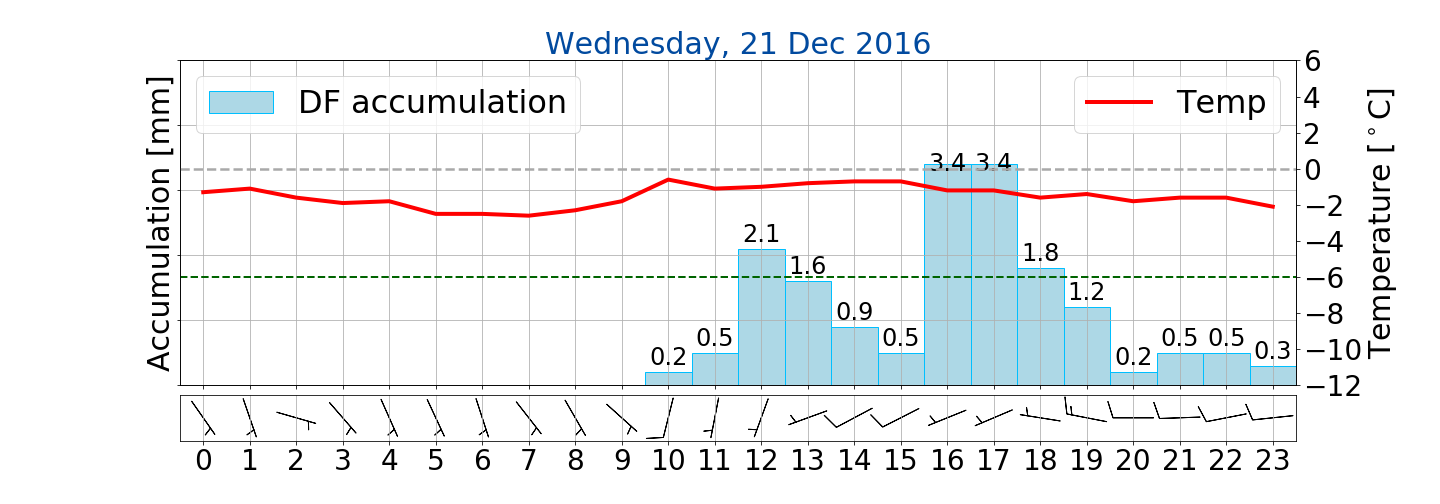
\includegraphics[trim={4.9cm 1.cm 1.5cm 1cm},clip,
% 		width=\textwidth]{./fig_weathermast/T_P_U_20161221}
% 		\caption{}\label{fig:TPU21}
% 	\end{subfigure}
% % \end{figure}
% % \begin{figure}\ContinuedFloat
% 	\centering
% 	%%%%%% 22/12
% 	\begin{subfigure}[b]{0.49\textwidth}
% 		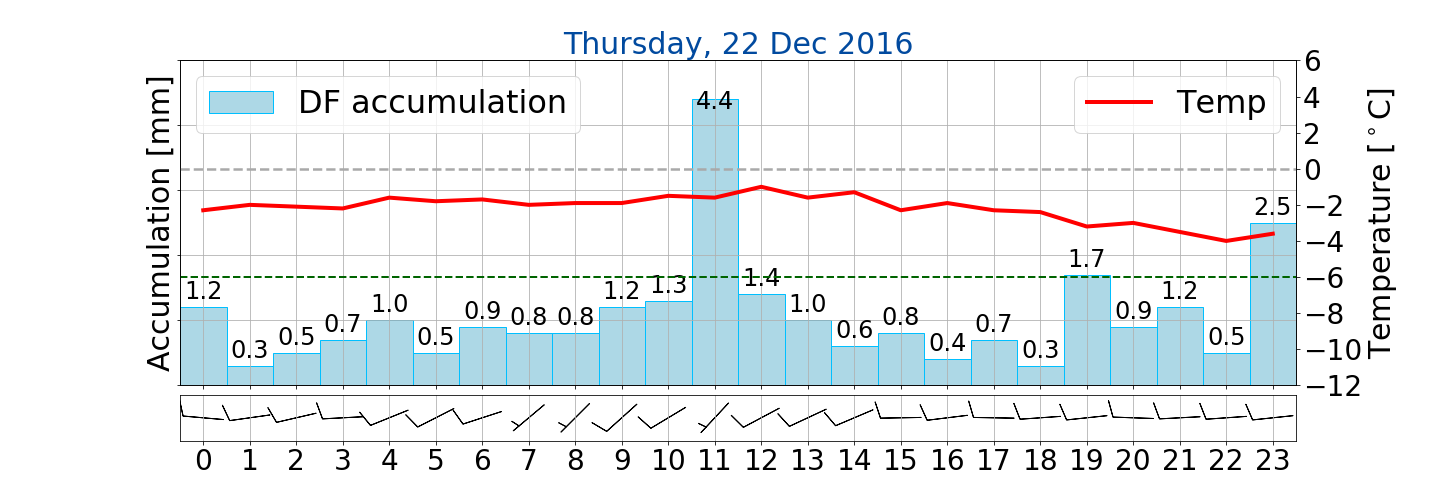
\includegraphics[trim={4.9cm 1.cm 1.5cm 1cm},clip,
% 		width=\textwidth]{./fig_weathermast/T_P_U_20161222}
% 		\caption{}\label{fig:TPU22}
% 	\end{subfigure}
% 	\hfill
% 	%%%%%% 23/12
% 	\begin{subfigure}[b]{0.49\textwidth}
% 		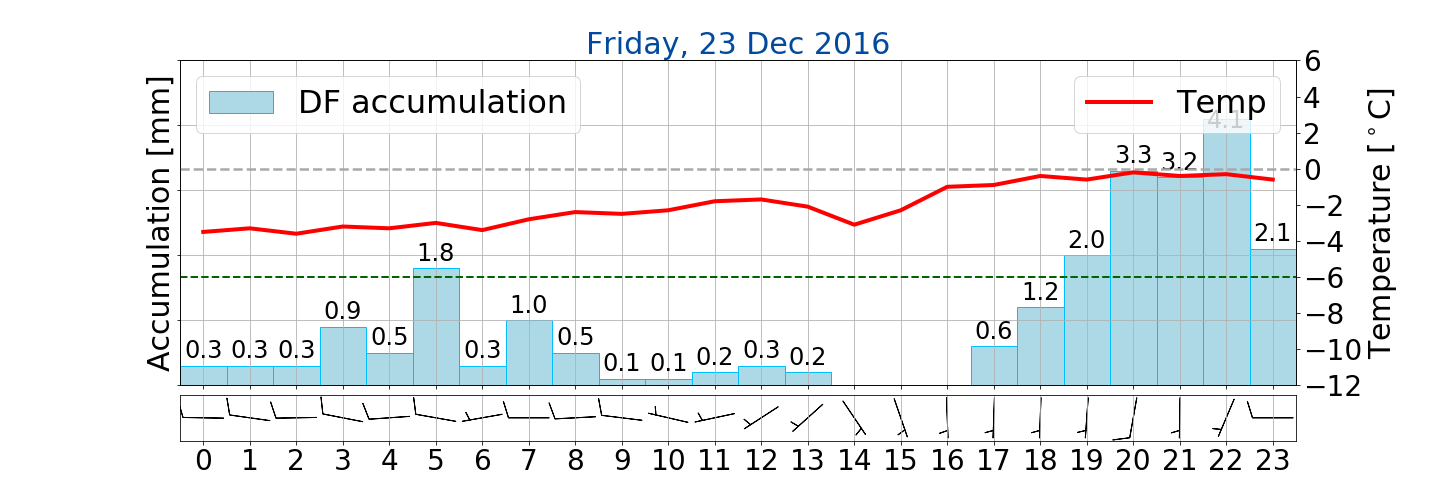
\includegraphics[trim={4.9cm 1.cm 1.5cm 1cm},clip,
% 		width=\textwidth]{./fig_weathermast/T_P_U_20161223}
% 		\caption{}\label{fig:TPU23}
% 	\end{subfigure}
% 	%\end{figure}
% 	%\begin{figure}[h]\ContinuedFloat
% 	%%%%%% 24/12
% 	\begin{subfigure}[b]{0.49\textwidth}
% 		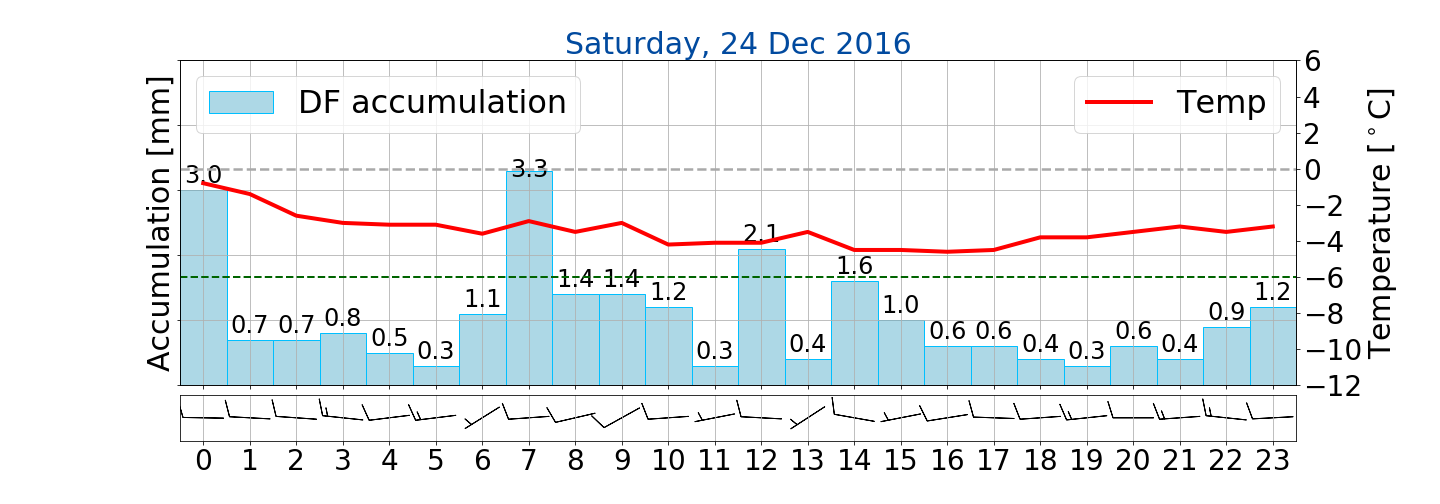
\includegraphics[trim={4.9cm 1.cm 1.5cm 1cm},clip,
% 		width=\textwidth]{./fig_weathermast/T_P_U_20161224}
% 		\caption{}\label{fig:TPU24}
% 	\end{subfigure}
% 	\hfill
% 	%%%%%% 25/12
% 	\begin{subfigure}[b]{0.49\textwidth}
% 		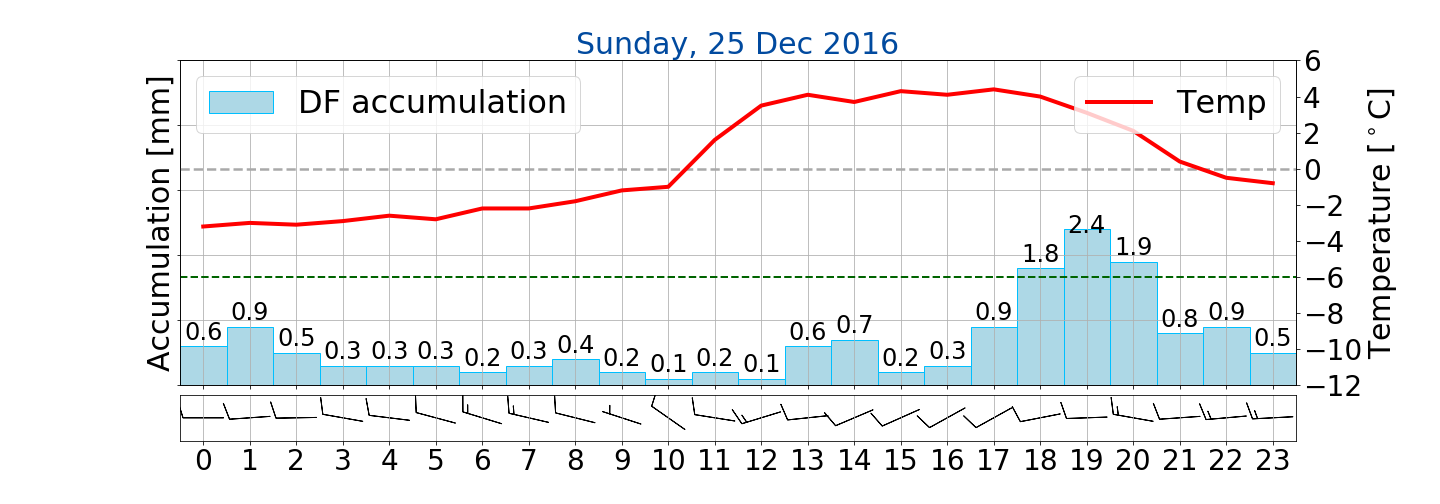
\includegraphics[trim={4.9cm 1.cm 1.5cm 1cm},clip,
% 		width=\textwidth]{./fig_weathermast/T_P_U_20161225}
% 		\caption{}\label{fig:TPU25}
% 	\end{subfigure}
%     %%%%%% 26/12
% 	\begin{subfigure}[b]{0.49\textwidth}
% 		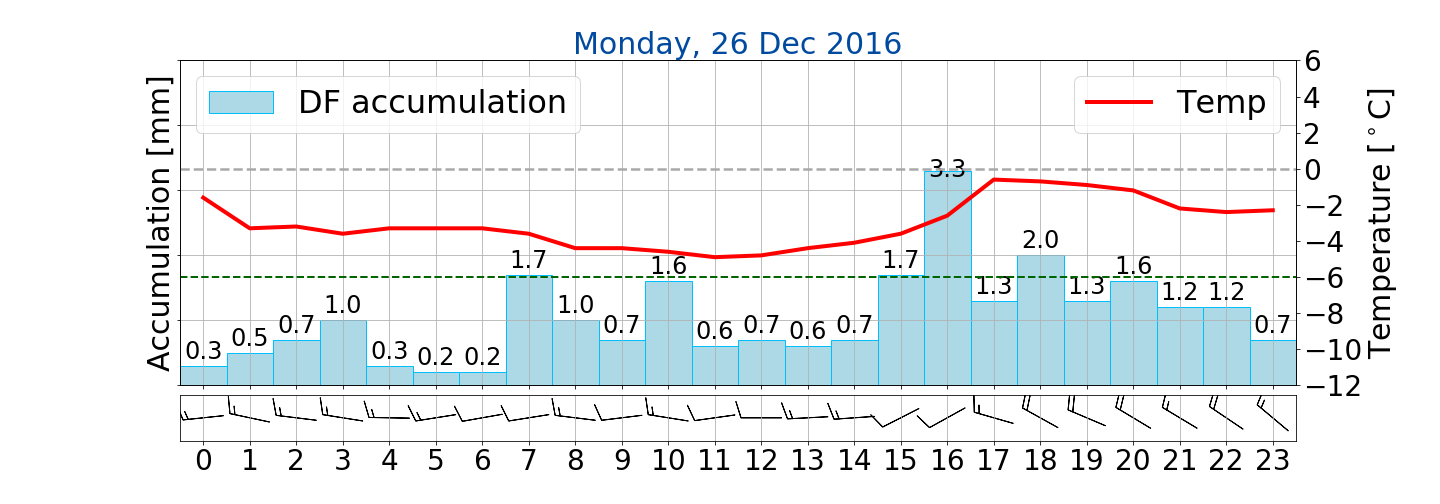
\includegraphics[trim={4.9cm 1.cm 1.5cm 1cm},clip,
% 		width=\textwidth]{./fig_weathermast/T_P_U_20161226}
% 		\caption{}\label{fig:TPU26}
% 	\end{subfigure}
%  \caption{Surface precipiation, temperature and wind observation from the weather mast at Haukeliseter during \num{21} and \SI{26}{\dec}. \SI{60}{\minute} total accumulation [\SI{}{\mm}] in light blue as bar, temperature (red, [\SI{}{\celsius}]), and wind as barbs [\SI{}{\mPs}]. Gray dashed line indicates the freezing temperature and the green dashed line the 30-year climate mean temperature at \SI{-6}{\celsius}. Hourly processed data taken from \cite{eklima_norwegian_2016}.} \label{fig:TPU}
%  \end{figure}
%  %%%%%%%%%%%%%%%%%%%%%%%%%%%%%%%%%%%%%%%%%%%%%%
% %The possible change of precipitation will be investigated with the temperature. 
% \noindent
% The temperature evolution will be used to investigate possible changes in the type of precipitation. 
% \\
% Snowfall is likely for temperatures up to \SI{2}{\celsius}. The intensity of the storm can be classified by the hourly averaged wind speed and direction as wind barbs in \SI{}{\mPs}.
% To understand which damage a storm can have, \cite{faeraas_urd_2016} released a table to associate wind strength with damage (see \Cref{tab:wind}).
% \\
% \Cref{fig:TPU21} shows a consistent temperature below \SI{0}{\celsius}. Cold air impinges on Scandinavia on \SI{21}{\dec} and because of the occluded cyclone influencing Norway (\Cref{fig:DT21}, \ref{fig:GP21}) frozen precipitation is observed at Haukeliseter. By \SI{12}{\UTC} on \SI{23}{\dec} an occluded front south of Iceland is influencing Norway. The occluded front is passing through Haukeliseter presented as an increase in precipitation. Because of a temperature change in \Cref{fig:TPU23} and the warm air influencing Norway (\Cref{fig:DT23}, \ref{fig:GP23}) mixed phase precipitation is assumed to occur. After the passage of the occluded front on \SI{23}{\dec} drop the observation of the \SI{2}{\metre} temperature at the measurement site (\Cref{fig:TPU24}). This 


\subsection{Surface comparison}\label{sec:res:large_scale_sfc}
%
%\textcolor{red}{What is the goal of this section?}
%\textcolor{red}{Insert here a general impression of observations and forecasts at Haukeli and relate it to the scatter plots}
The large scale weather situation was discussed in \Cref{sec:largeScale}. It has shown, that two low pressure systems affecte Norway around Christmas 2016. \Cref{fig:res:sfc_obs_meps} display the observations and intialisations for pressure, temperature, wind, and precipitation on \num{21} to \SI{27}{\dec}. 
\\
A comparison between the surface observations at Haukeliseter and the ECMWF analysis of the dynamic tropopause and geopotential thickness maps show that frontal transitions occurred on three days during the 2016 Christmas storm, \num{23}, \num{25}, and \SI{26}{\dec} (\Cref{sec:largeScale}). 
These show in the measurements and MEPS ensemble forecasts on \num{23}, \num{25}, and \SI{26}{\dec} (\Cref{fig:res:sfc_obs_meps}).
\\
\Cref{fig:res:sfc_obs_meps} shows the different parameters forecasts initialised at \SI{00}{\UTC} for \num{23}, \num{25}, and \SI{26}{\dec}, as well as the observations at the Haukeliseter measurement site. During all days the MEPS forecast seems to be able to predict similar pressure, temperature, wind, and precipitation as is observed. Overestimations are seen for wind speed and surface precipiation amount in \Cref{fig:res:sfc_wd21}, \subref{fig:res:sfc_wd23}, \subref{fig:res:sfc_wd25}, \subref{fig:res:sfc_wd26}, \subref{fig:res:sfc_precip21}, \subref{fig:res:sfc_precip23},\subref{fig:res:sfc_precip25}, and \subref{fig:res:sfc_precip26}. 
\\
%
%%%%%%% image sfc obs  %%%%%%%%%%%%%%%%
\begin{figure}[H]
	\centering
	% sfc pressure
	\begin{subfigure}[b]{0.75\textwidth}
		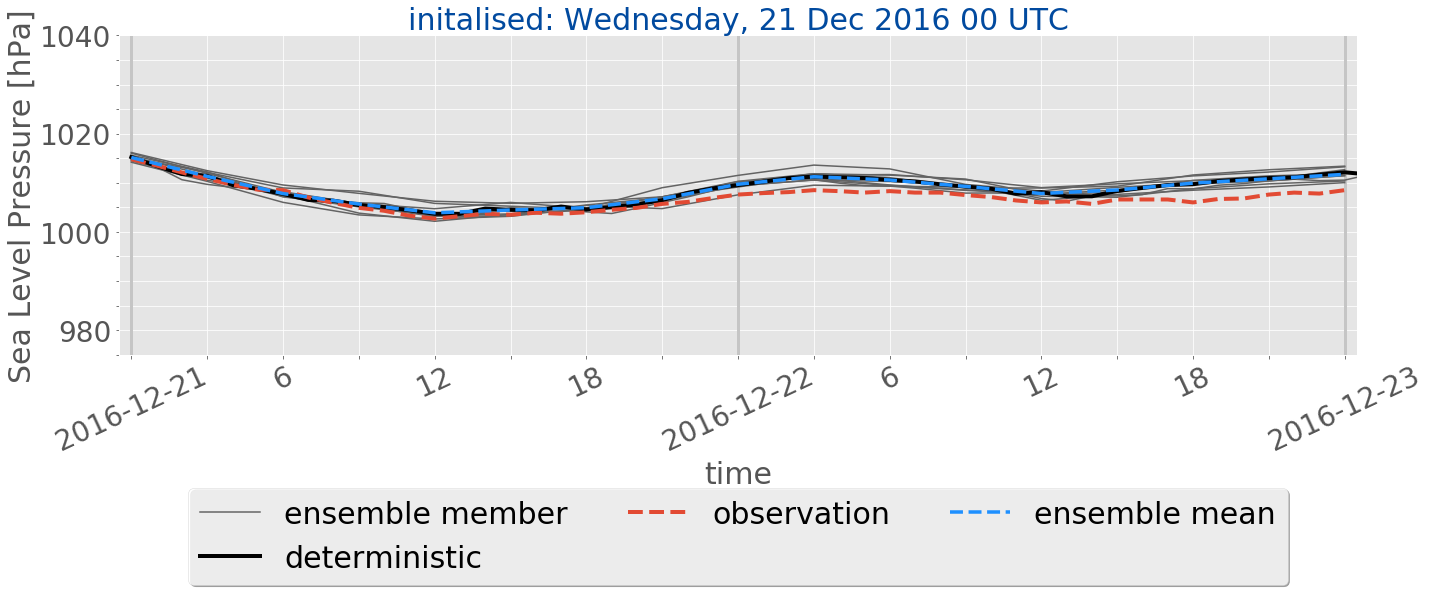
\includegraphics[trim={0.cm 1.5cm 0cm 0cm},clip,
		width=\textwidth]{./fig_sfc_pressure/20161221_00}
		\caption{}\label{fig:res:sfc_pres21}
	\end{subfigure}
	% sfc temp
	\begin{subfigure}[b]{0.75\textwidth}
		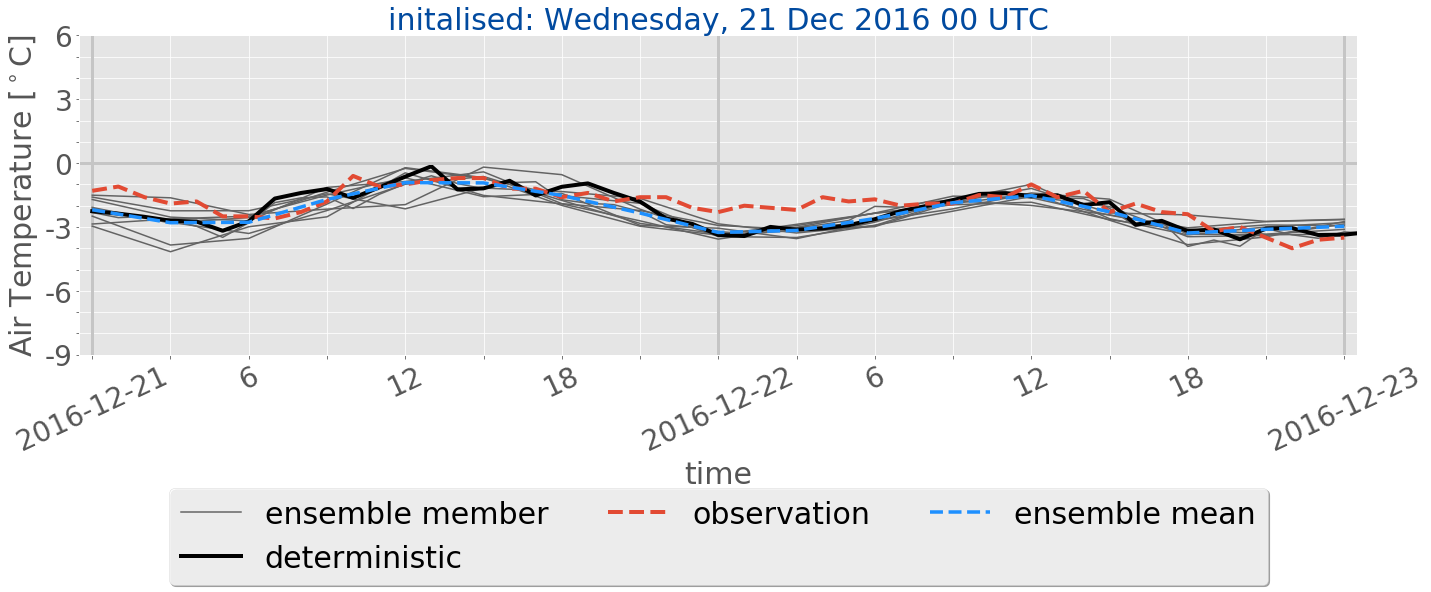
\includegraphics[trim={0.cm 1.5cm 0cm 0cm},clip,
		width=\textwidth]{./fig_sfc_temp/20161221_00}
		\caption{}\label{fig:res:sfc_temp21}
	\end{subfigure}
	%
	% sfc wd
	\begin{subfigure}[b]{0.75\textwidth}
		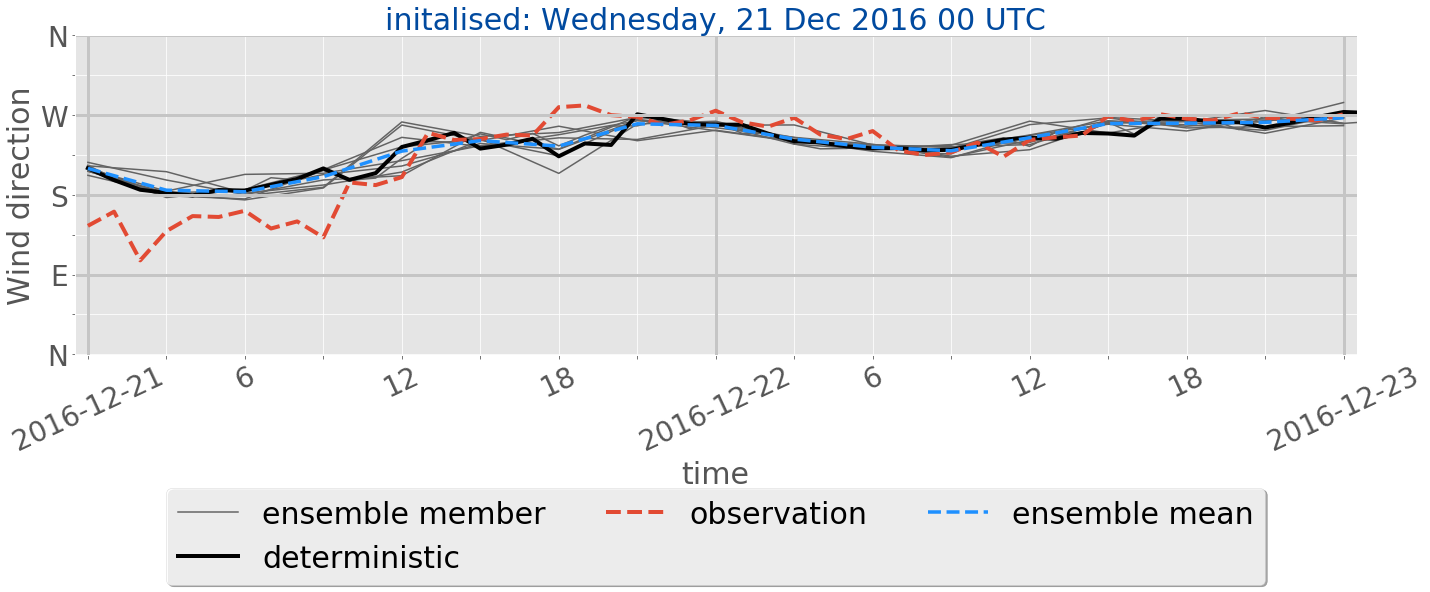
\includegraphics[trim={0.cm 1.5cm 0cm 0cm},clip,
		width=\textwidth]{./fig_sfc_wd/20161221_00}
		\caption{}\label{fig:res:sfc_wd21}
	\end{subfigure}
	% sfc ws
	\begin{subfigure}[b]{0.75\textwidth}
		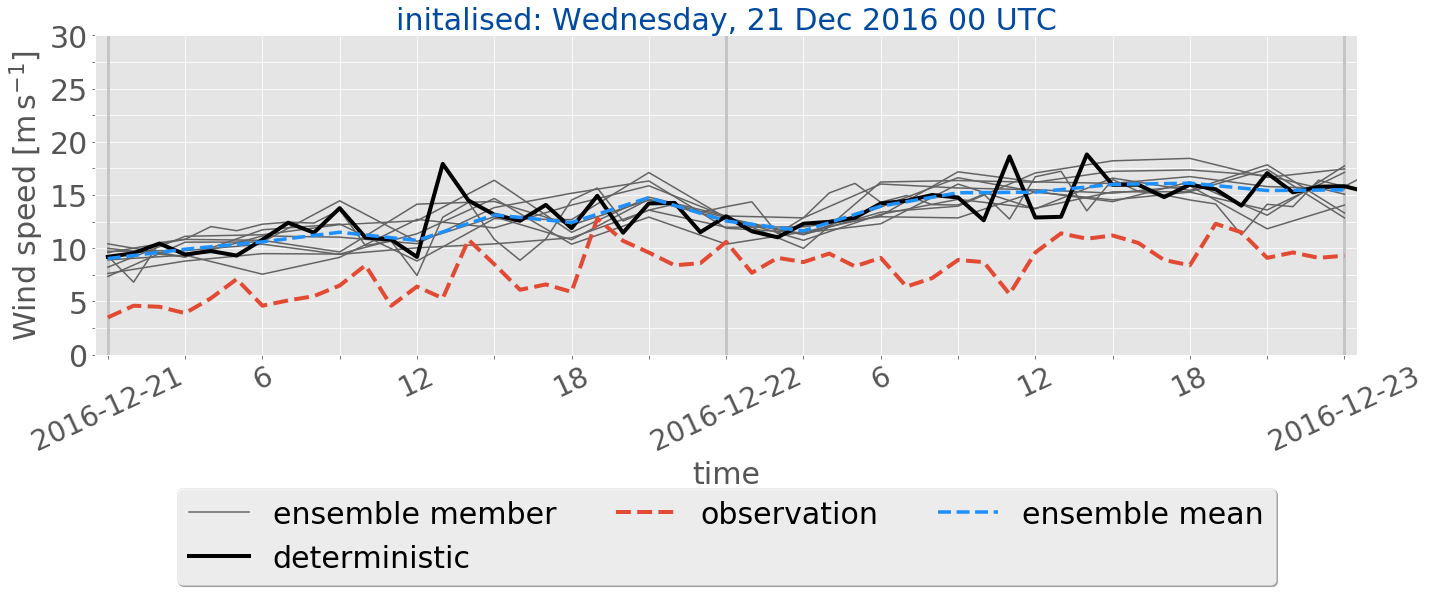
\includegraphics[trim={0.cm 1.5cm 0cm 0cm},clip,
		width=\textwidth]{./fig_sfc_ws/20161221_00}
		\caption{}\label{fig:res:sfc_ws21}
	\end{subfigure}
	% sfc precip
	\begin{subfigure}[b]{0.75\textwidth}
		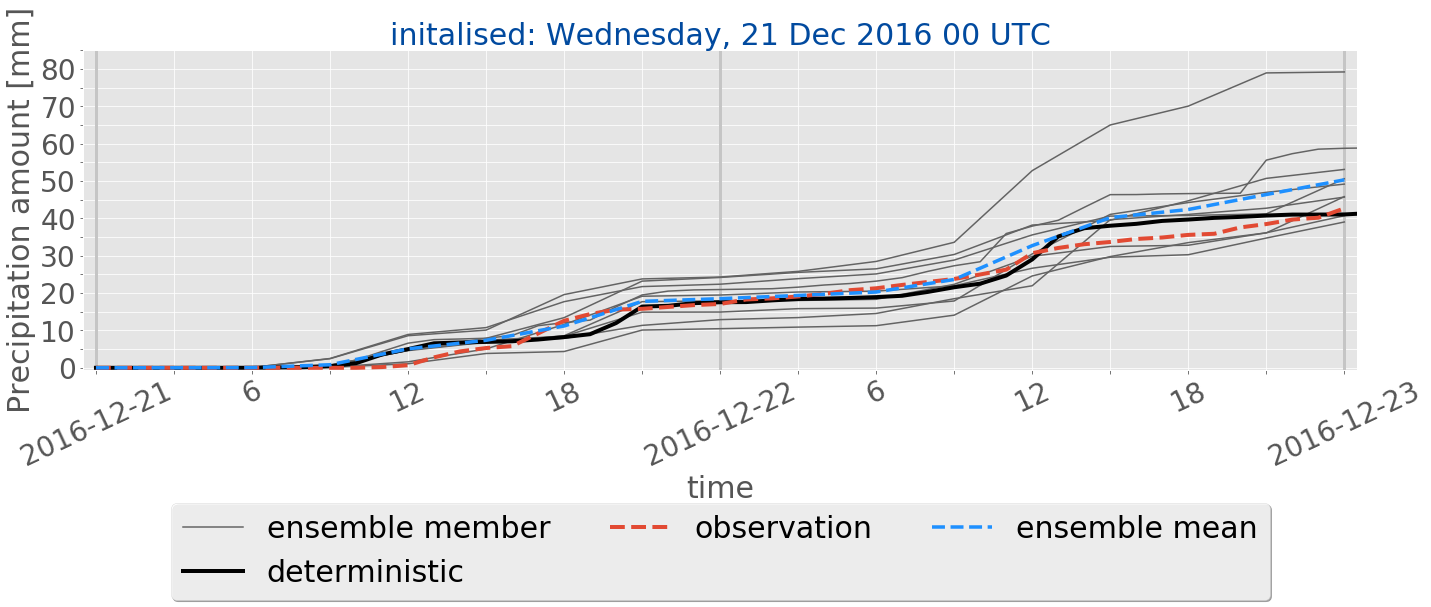
\includegraphics[trim={0.cm 1.5cm 0cm 0cm},clip,
		width=\textwidth]{./fig_sfc_precip/20161221_00}
		\caption{}\label{fig:res:sfc_precip21}
	\end{subfigure}
	% label
	\begin{subfigure}[b]{0.8\textwidth}
		\centering
		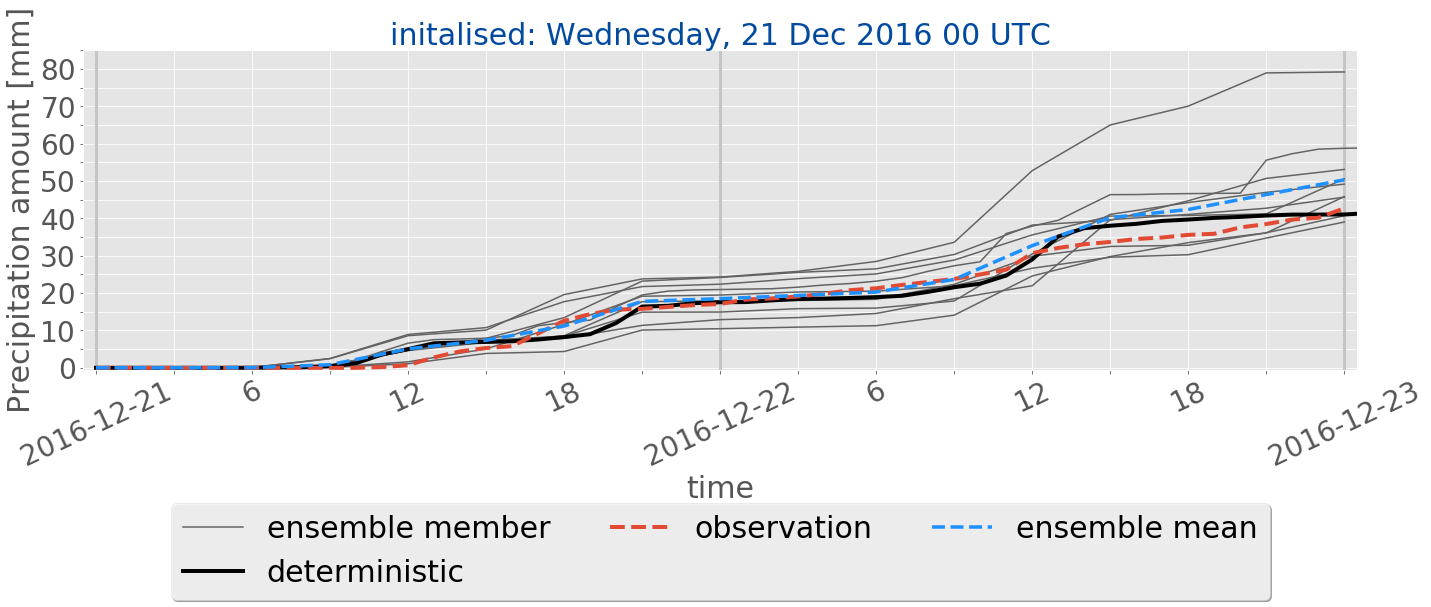
\includegraphics[trim={5.5cm 0cm 5.cm 17.7cm},clip,
		width=0.8\textwidth]{./fig_sfc_precip/20161221_00_label}
	\end{subfigure}
    \caption{\SI{48}{\hour} surface observations and MEPS ensemble forecasts initialised on \SI{21}{\dec} at \SI{0}{\UTC}. 
%     (\protect\subref{fig:res:sfc_pres21}, \protect\subref{fig:res:sfc_temp21}, \protect\subref{fig:res:sfc_wd21}, \protect\subref{fig:res:sfc_ws21}, \protect\subref{fig:res:sfc_precip21})
%     , \SI{23}{\dec} at \SI{0}{\UTC} (\protect\subref{fig:res:sfc_pres23}, \protect\subref{fig:res:sfc_temp23}, \protect\subref{fig:res:sfc_wd23}, \protect\subref{fig:res:sfc_ws23}, \protect\subref{fig:res:sfc_precip23}), and on \SI{25}{\dec} at \SI{0}{\UTC} (\protect\subref{fig:res:sfc_pres25}, \protect\subref{fig:res:sfc_temp25}, \protect\subref{fig:res:sfc_wd25}, \protect\subref{fig:res:sfc_ws25}, \protect\subref{fig:res:sfc_precip25}) as well as \SI{26}{\dec} (\protect\subref{fig:res:sfc_pres26}, \protect\subref{fig:res:sfc_temp26}, \protect\subref{fig:res:sfc_wd26}, \protect\subref{fig:res:sfc_ws26}, \protect\subref{fig:res:sfc_precip26}). 
Line representation according to the label. Upper to low panel: sea level pressure, \SI{2}{\metre} air temperature, \SI{10}{\metre} wind direction and speed, and precipitation amount. \textit{Continued on next page.}}\label{fig:res:sfc_obs_meps}
	%
\end{figure}
\begin{figure}[H]\ContinuedFloat
	\centering
	% sfc pressure
	\begin{subfigure}[b]{0.75\textwidth}
		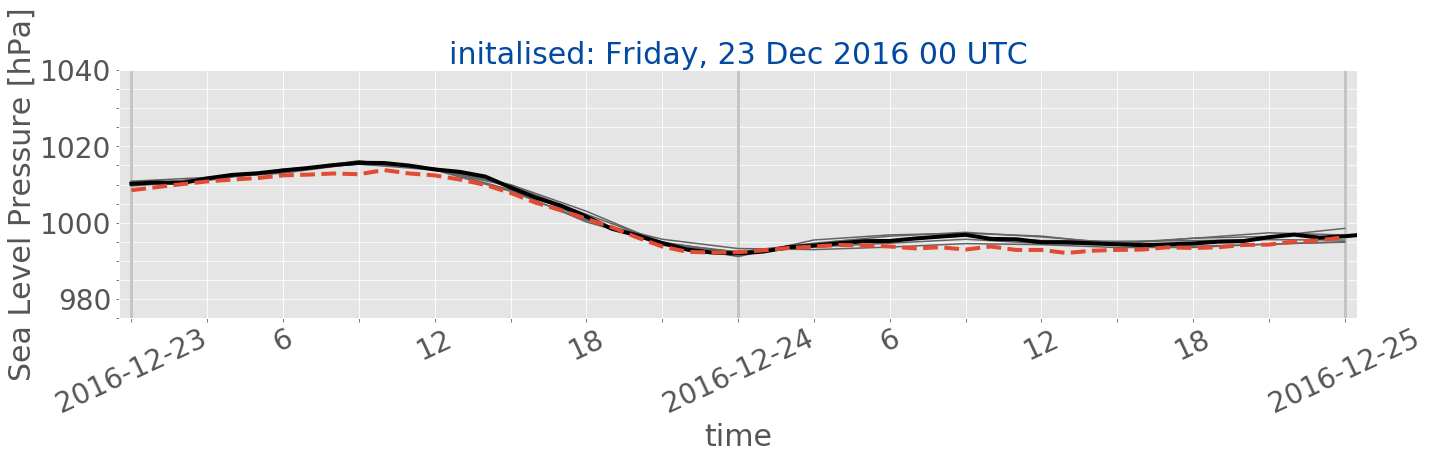
\includegraphics[trim={0.cm 1.5cm 0cm 0cm},clip,
		width=\textwidth]{./fig_sfc_pressure/20161223_00}
		\caption{}\label{fig:res:sfc_pres23}
	\end{subfigure}
	% sfc temp
	\begin{subfigure}[b]{0.75\textwidth}
		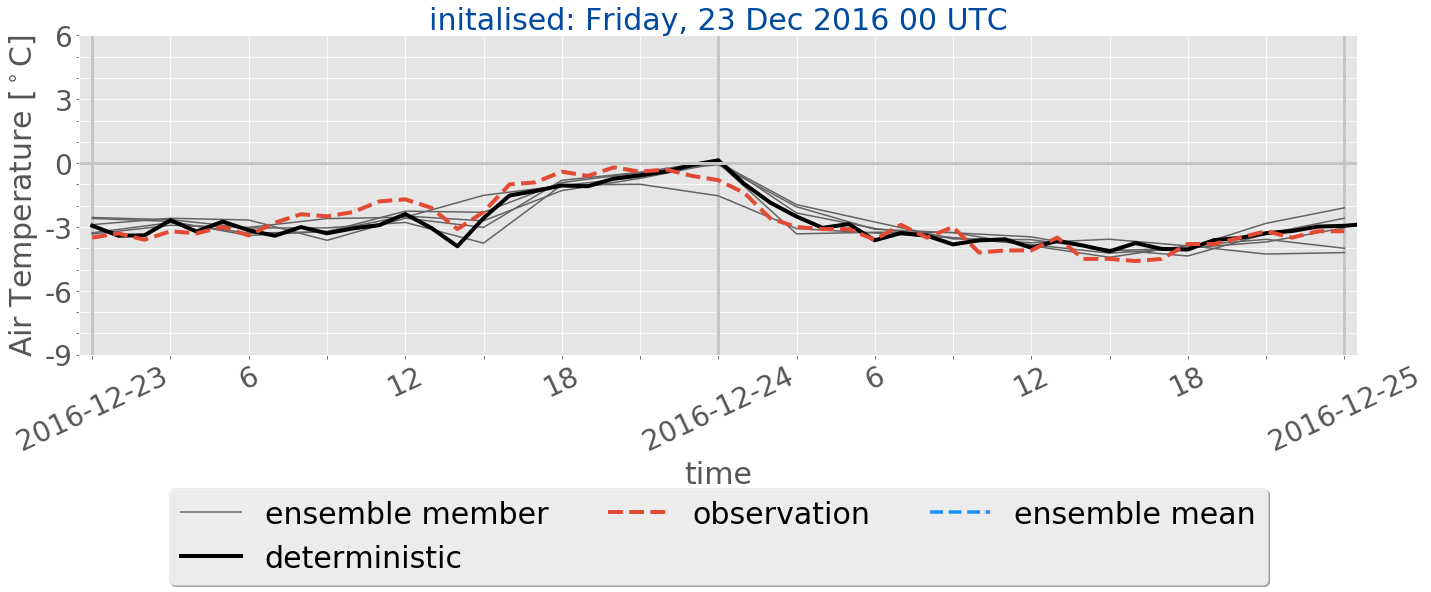
\includegraphics[trim={0.cm 1.5cm 0cm 0cm},clip,
		width=\textwidth]{./fig_sfc_temp/20161223_00}
		\caption{}\label{fig:res:sfc_temp23}
	\end{subfigure}
	%
	% sfc wd
	\begin{subfigure}[b]{0.75\textwidth}
		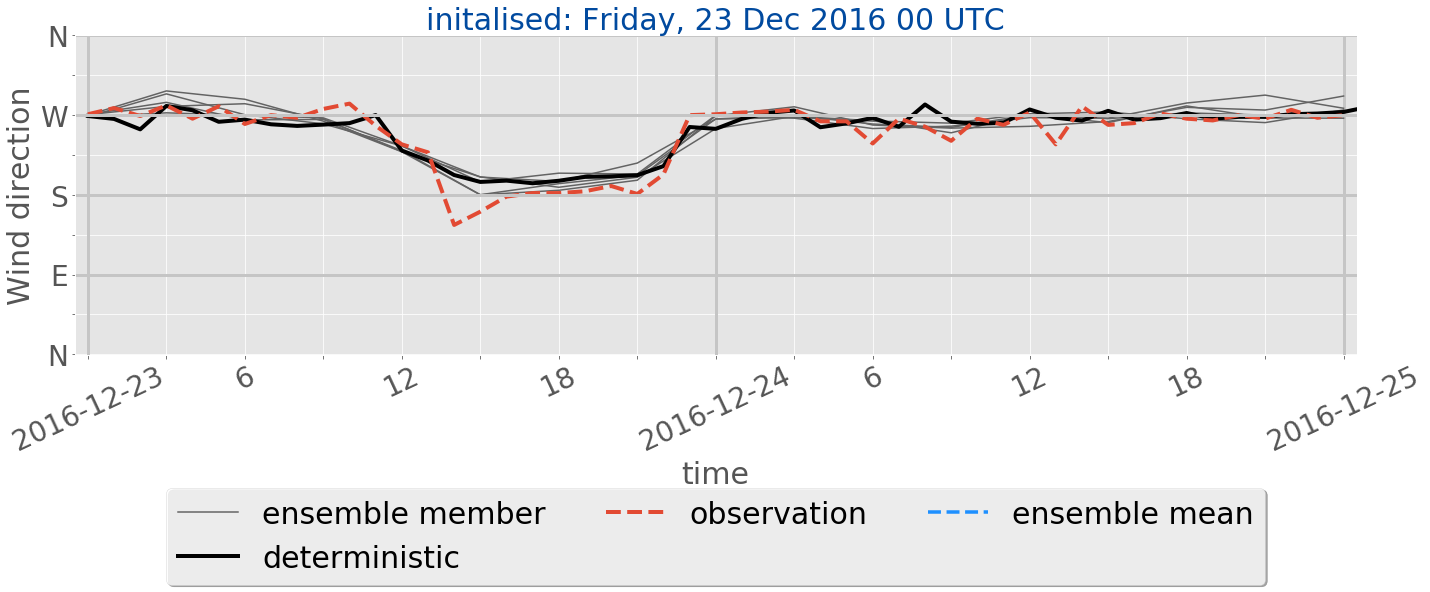
\includegraphics[trim={0.cm 1.5cm 0cm 0cm},clip,
		width=\textwidth]{./fig_sfc_wd/20161223_00}
		\caption{}\label{fig:res:sfc_wd23}
	\end{subfigure}
	% sfc ws
	\begin{subfigure}[b]{0.75\textwidth}
		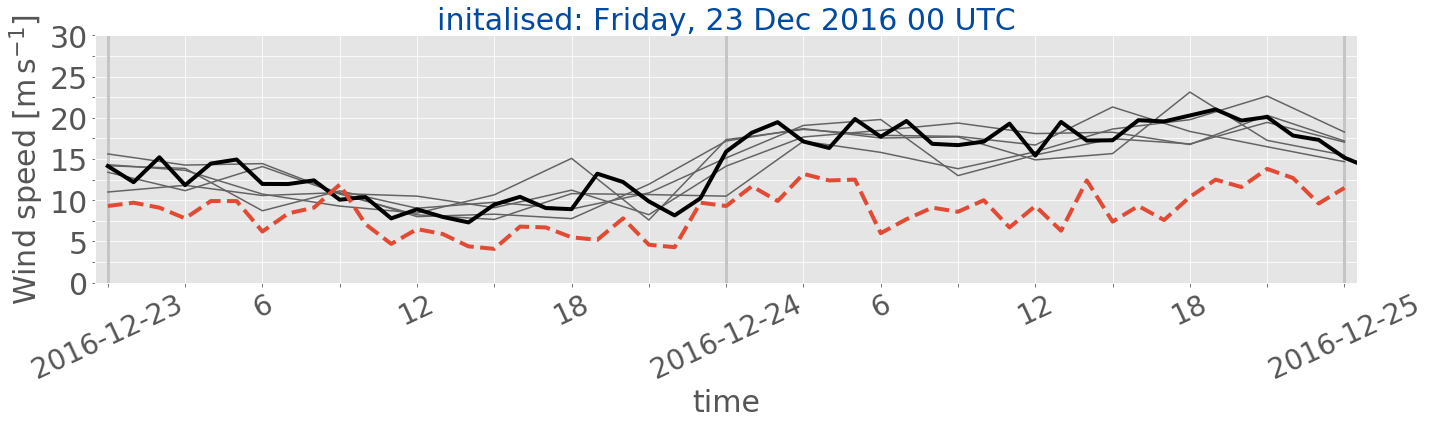
\includegraphics[trim={0.cm 1.5cm 0cm 0cm},clip,
		width=\textwidth]{./fig_sfc_ws/20161223_00}
		\caption{}\label{fig:res:sfc_ws23}
	\end{subfigure}
	% sfc precip
	\begin{subfigure}[b]{0.75\textwidth}
		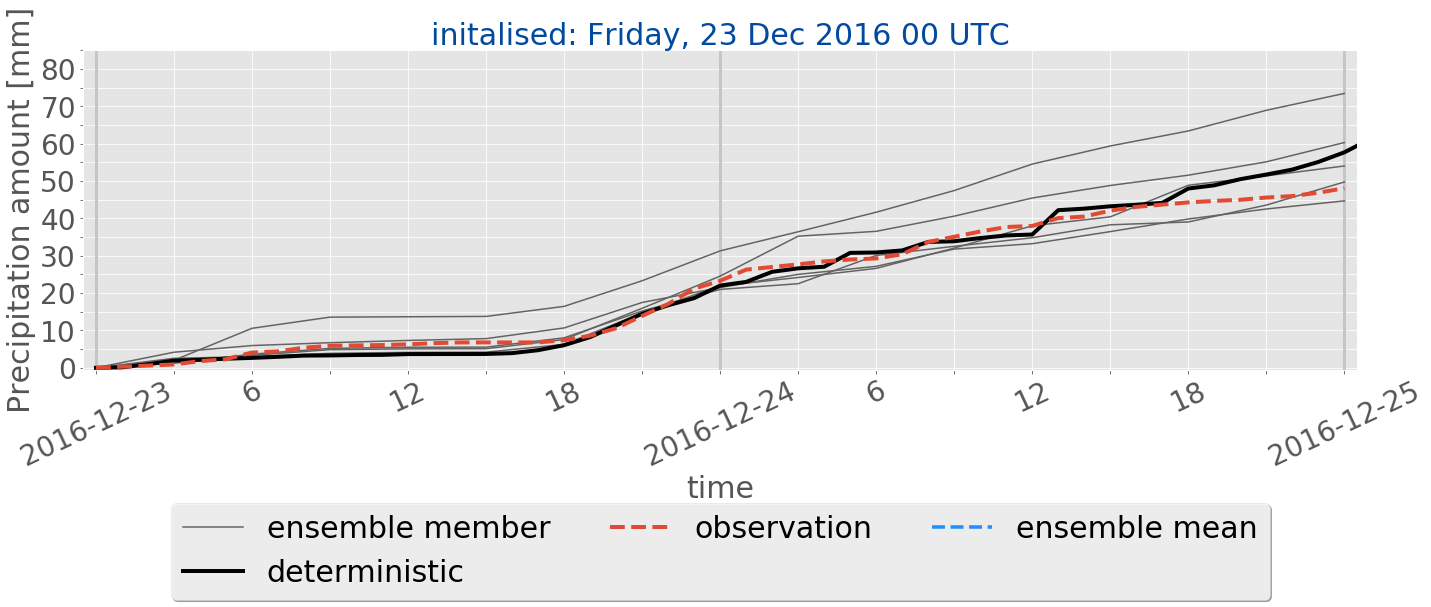
\includegraphics[trim={0.cm 1.5cm 0cm 0cm},clip,
		width=\textwidth]{./fig_sfc_precip/20161223_00}
		\caption{}\label{fig:res:sfc_precip23}
	\end{subfigure}
	% label
	\begin{subfigure}[b]{0.8\textwidth}
		\centering
		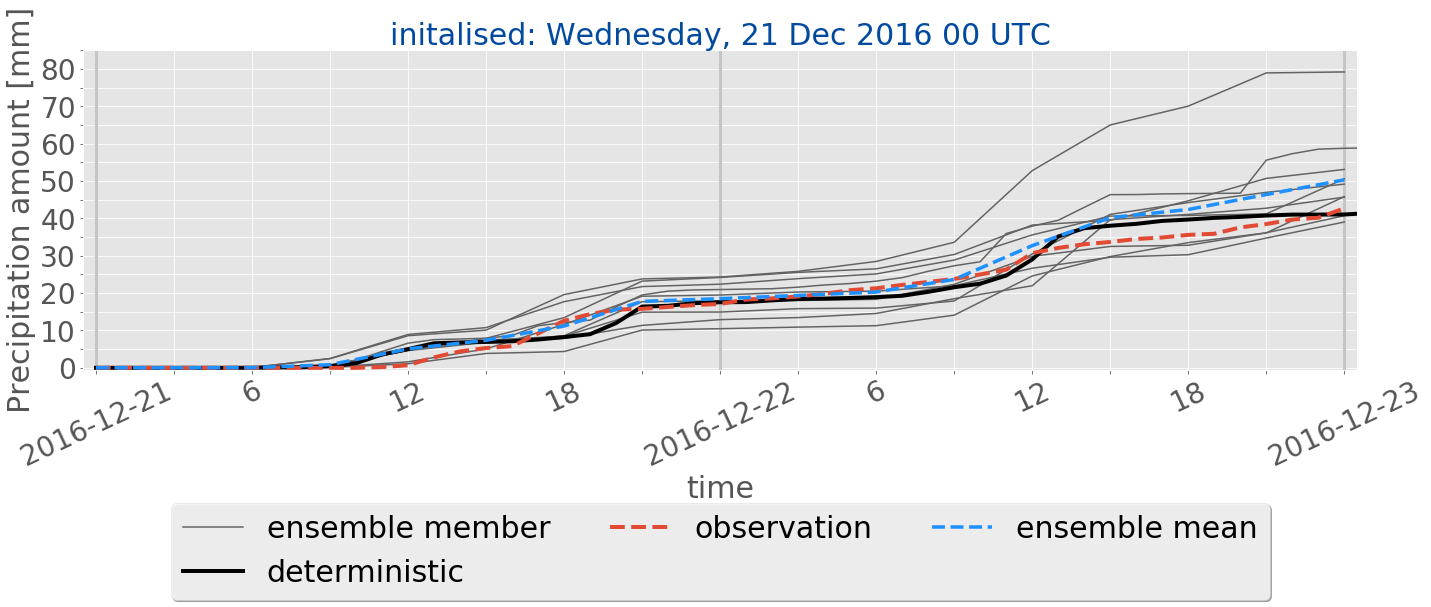
\includegraphics[trim={5.5cm 0cm 5.cm 17.7cm},clip,
		width=0.8\textwidth]{./fig_sfc_precip/20161221_00_label}
	\end{subfigure}
    \caption{\textit{(Continued from previous page.)} Initialisation on \SI{23}{\dec} at \SI{0}{\UTC}. }
	%
\end{figure}
%
\begin{figure}[H]\ContinuedFloat
	\centering
	% sfc pressure
	%
	\begin{subfigure}[b]{0.75\textwidth}
		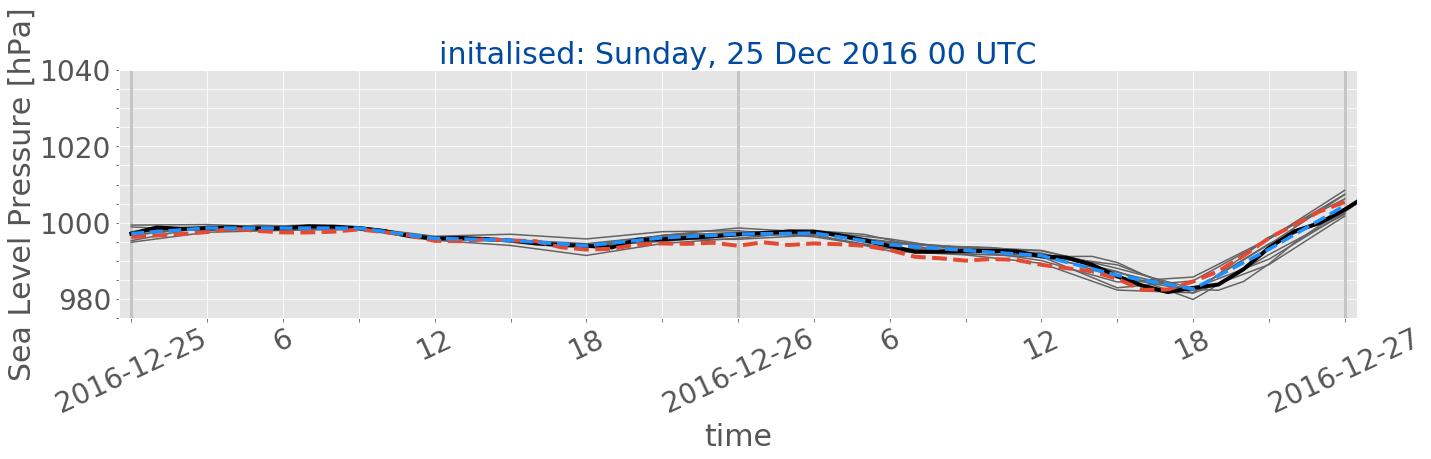
\includegraphics[trim={0.cm 1.5cm 0cm 0cm},clip,
		width=\textwidth]{./fig_sfc_pressure/20161225_00}
		\caption{}\label{fig:res:sfc_pres25}
	\end{subfigure}
	% sfc temp
	%
	\begin{subfigure}[b]{0.75\textwidth}
		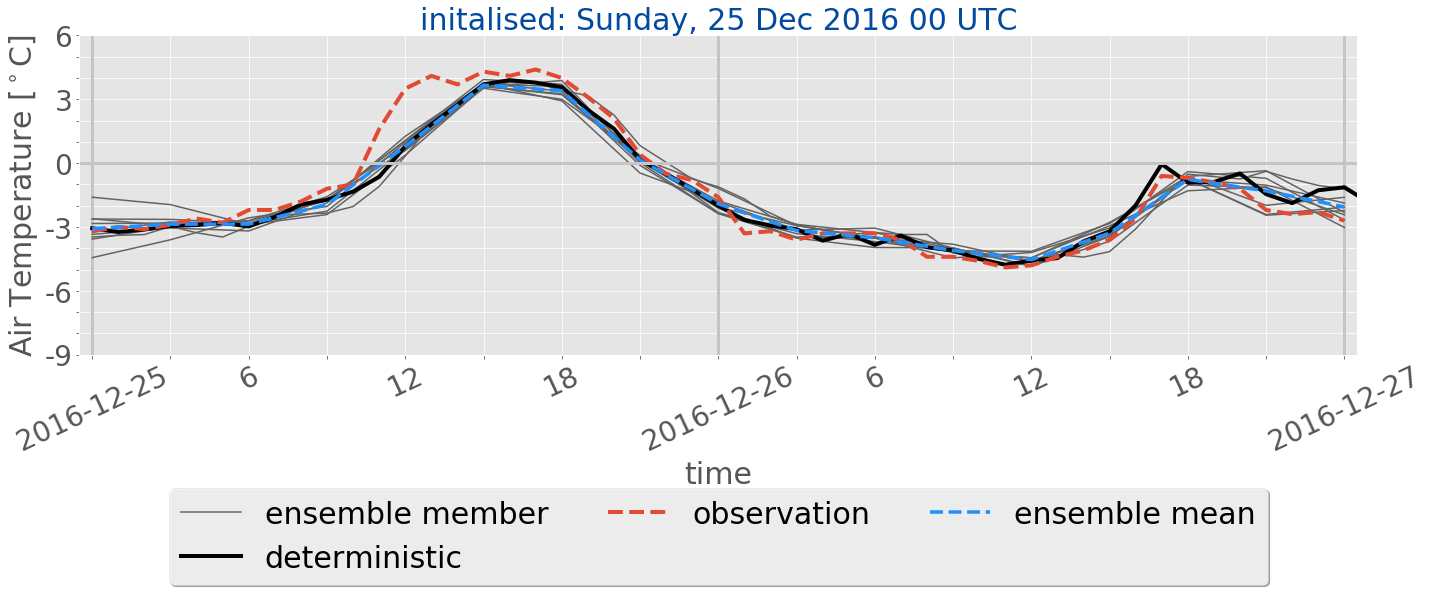
\includegraphics[trim={0.cm 1.5cm 0cm 0cm},clip,
		width=\textwidth]{./fig_sfc_temp/20161225_00}
		\caption{}\label{fig:res:sfc_temp25}
	\end{subfigure}
	% sfc wd
	%
	\begin{subfigure}[b]{0.75\textwidth}
		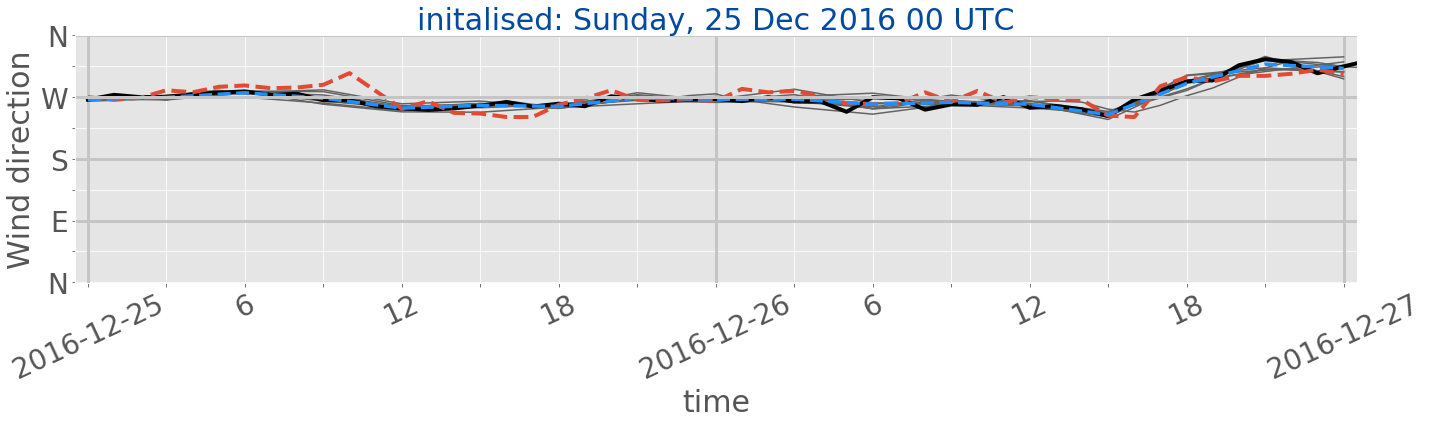
\includegraphics[trim={0.cm 1.5cm 0cm 0cm},clip,
		width=\textwidth]{./fig_sfc_wd/20161225_00}
		\caption{}\label{fig:res:sfc_wd25}
	\end{subfigure}
	% sfc ws
	%
	\begin{subfigure}[b]{0.75\textwidth}
		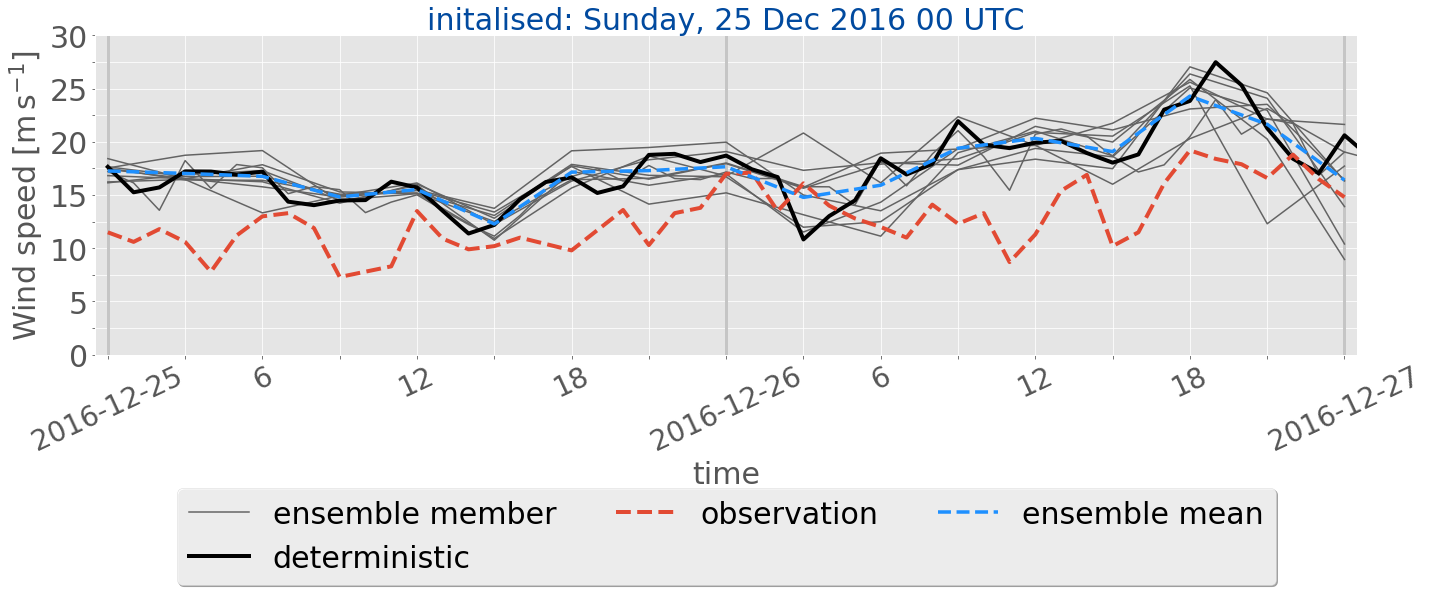
\includegraphics[trim={0.cm 1.5cm 0cm 0cm},clip,
		width=\textwidth]{./fig_sfc_ws/20161225_00}
		\caption{}\label{fig:res:sfc_ws25}
	\end{subfigure}
	% sfc precip
	%
	\begin{subfigure}[b]{0.75\textwidth}
		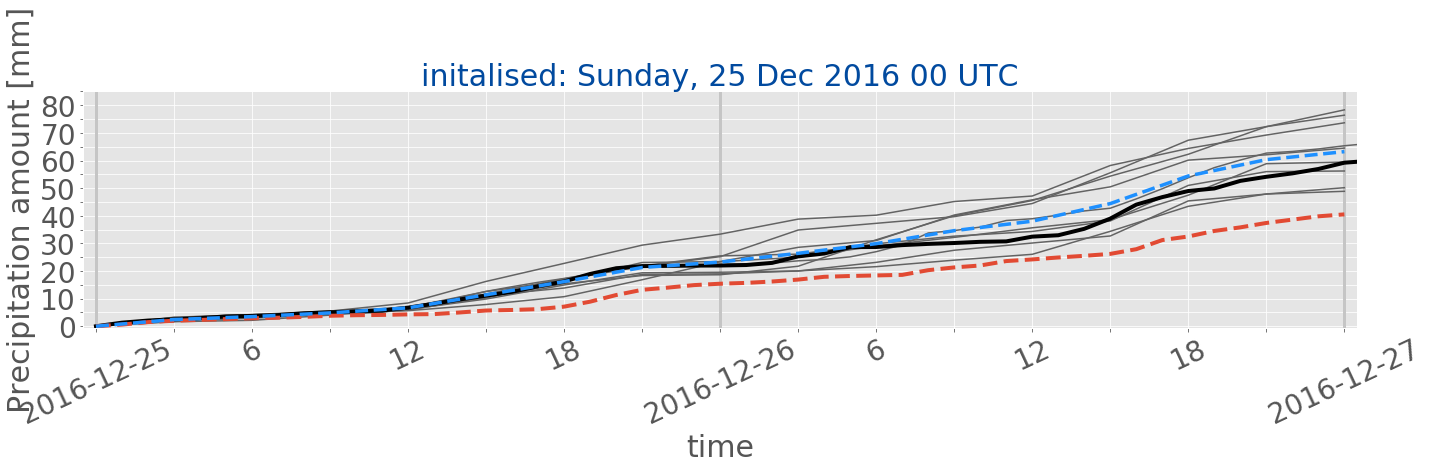
\includegraphics[trim={0.cm 1.5cm 0cm 0cm},clip,
		width=\textwidth]{./fig_sfc_precip/20161225_00}
		\caption{}\label{fig:res:sfc_precip25}
	\end{subfigure}
	% label
	\begin{subfigure}[b]{0.8\textwidth}
		\centering
		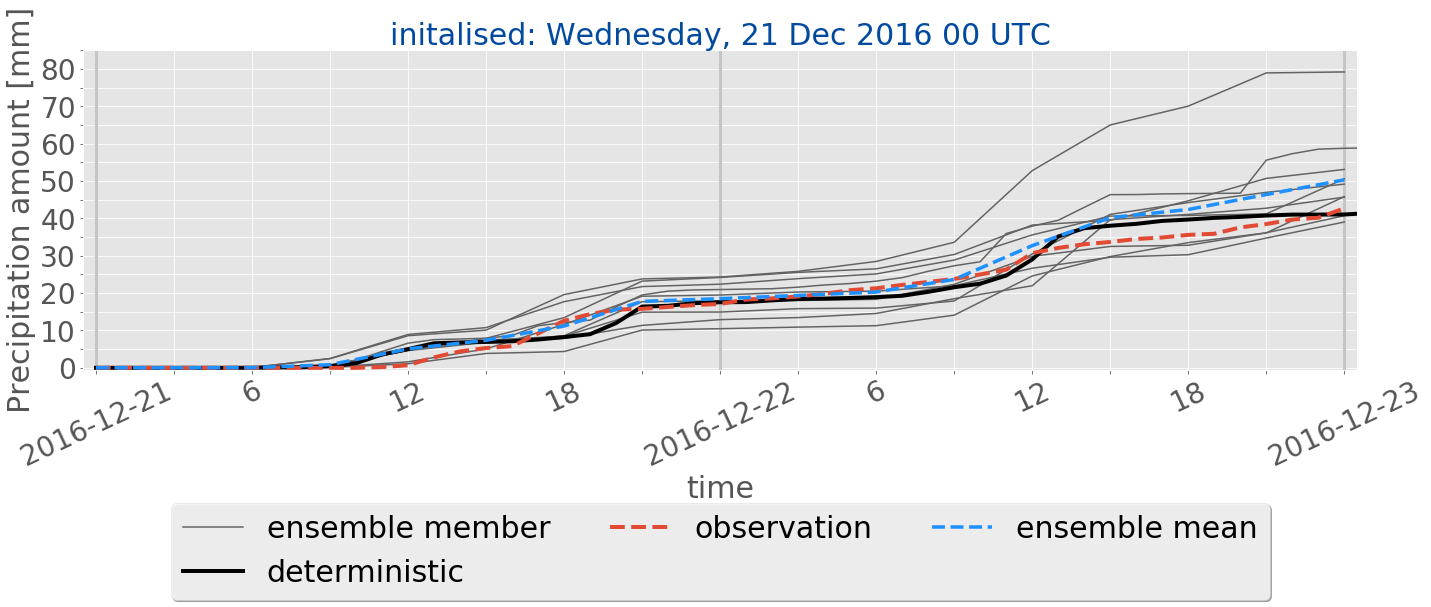
\includegraphics[trim={5.5cm 0cm 5.cm 17.7cm},clip,
		width=0.8\textwidth]{./fig_sfc_precip/20161221_00_label}
	\end{subfigure}
    \caption{\textit{(Continued from previous page.)} Initialisation on \SI{25}{\dec} at \SI{0}{\UTC}.}
	%
\end{figure}
%
\begin{figure}[H]\ContinuedFloat
	\centering
	% sfc pressure
	\begin{subfigure}[b]{0.75\textwidth}
		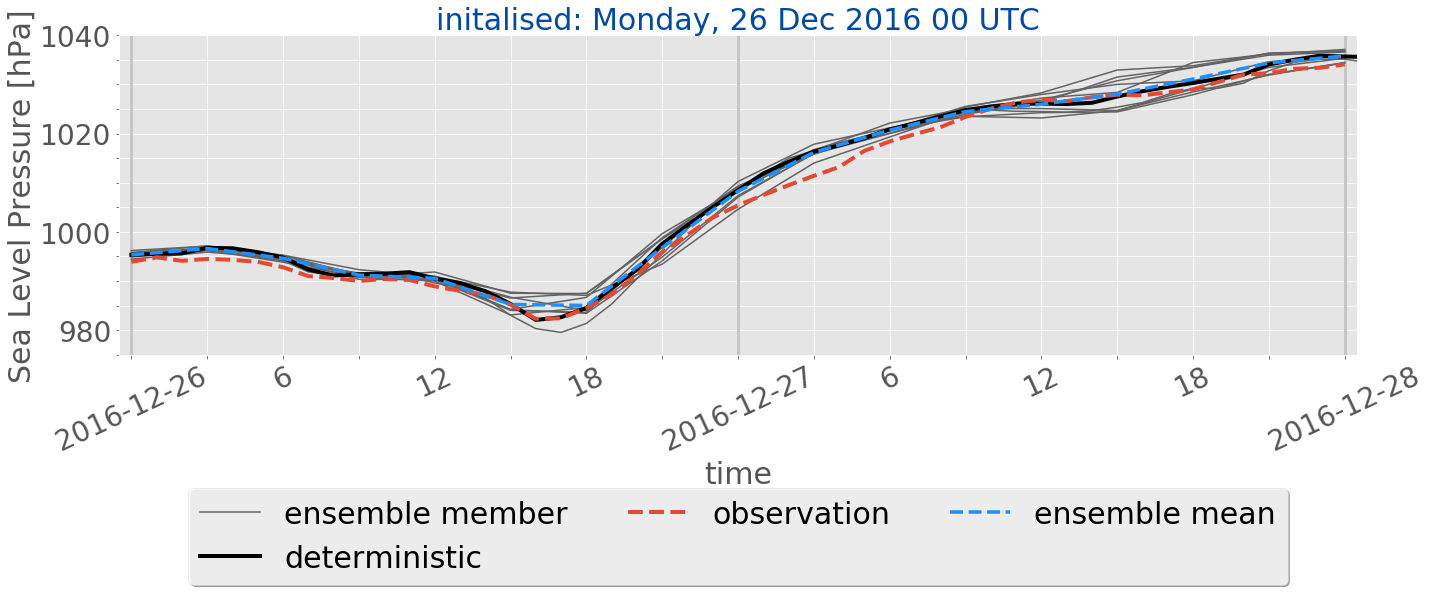
\includegraphics[trim={0.cm 1.5cm 0cm 0cm},clip,
		width=\textwidth]{./fig_sfc_pressure/20161226_00}
		\caption{}\label{fig:res:sfc_pres26}
	\end{subfigure}
	
	% sfc temp
	\begin{subfigure}[b]{0.75\textwidth}
		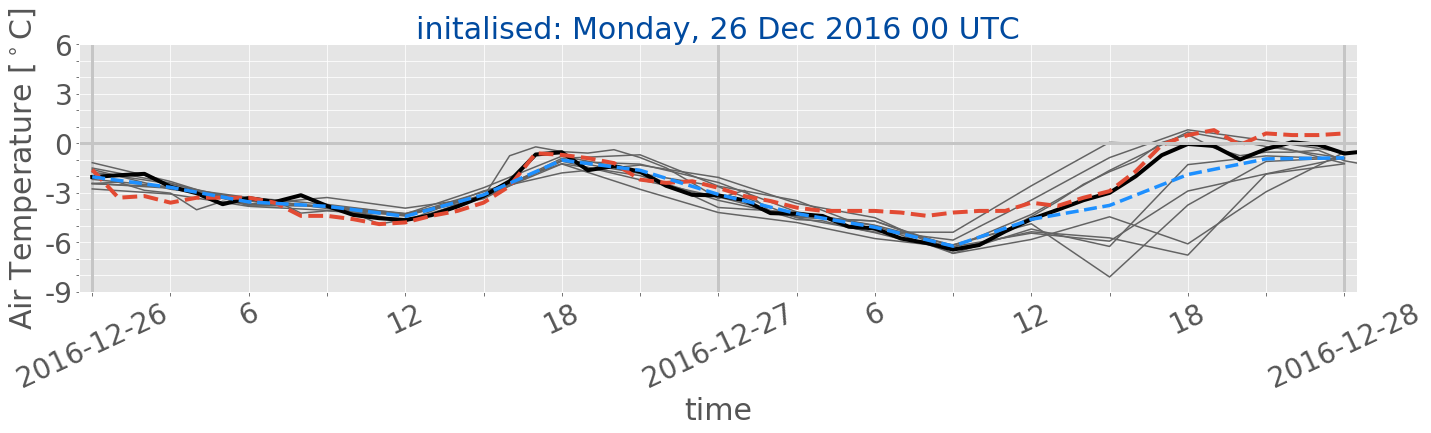
\includegraphics[trim={0.cm 1.5cm 0cm 0cm},clip,
		width=\textwidth]{./fig_sfc_temp/20161226_00}
		\caption{}\label{fig:res:sfc_temp26}
	\end{subfigure}
	
	% sfc wd
	\begin{subfigure}[b]{0.75\textwidth}
		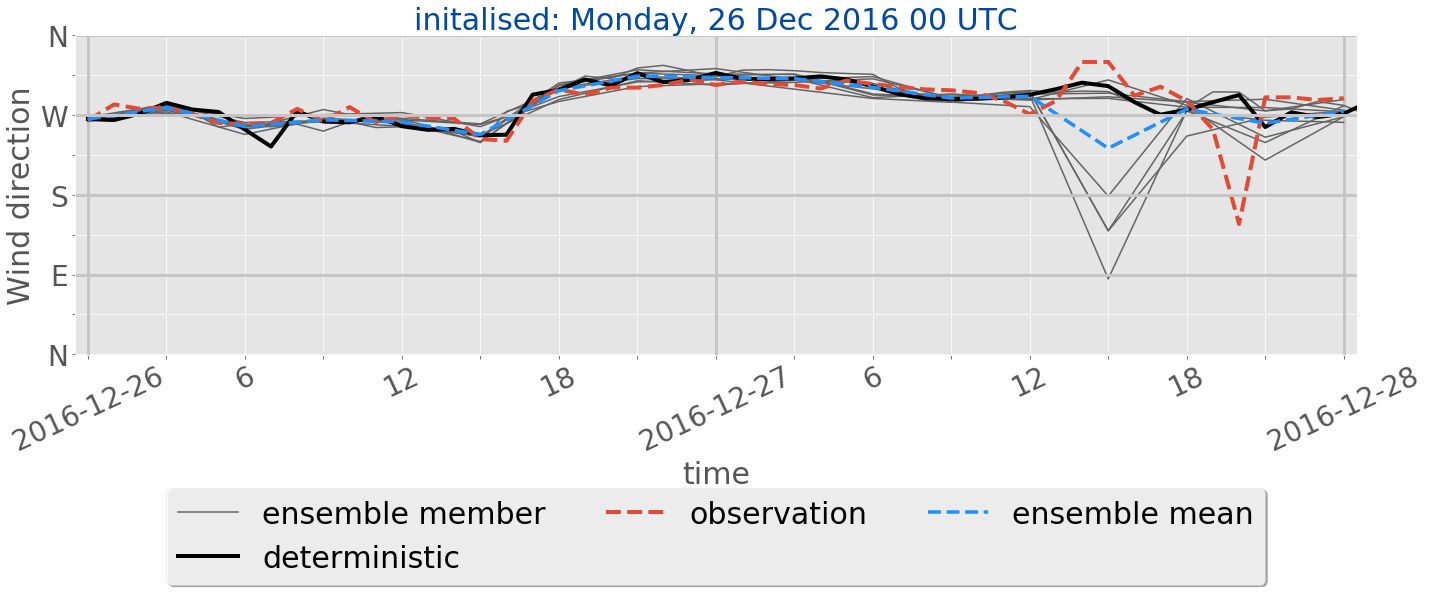
\includegraphics[trim={0.cm 1.5cm 0cm 0cm},clip,
		width=\textwidth]{./fig_sfc_wd/20161226_00}
		\caption{}\label{fig:res:sfc_wd26}
	\end{subfigure}
	
	% sfc ws
	\begin{subfigure}[b]{0.75\textwidth}
		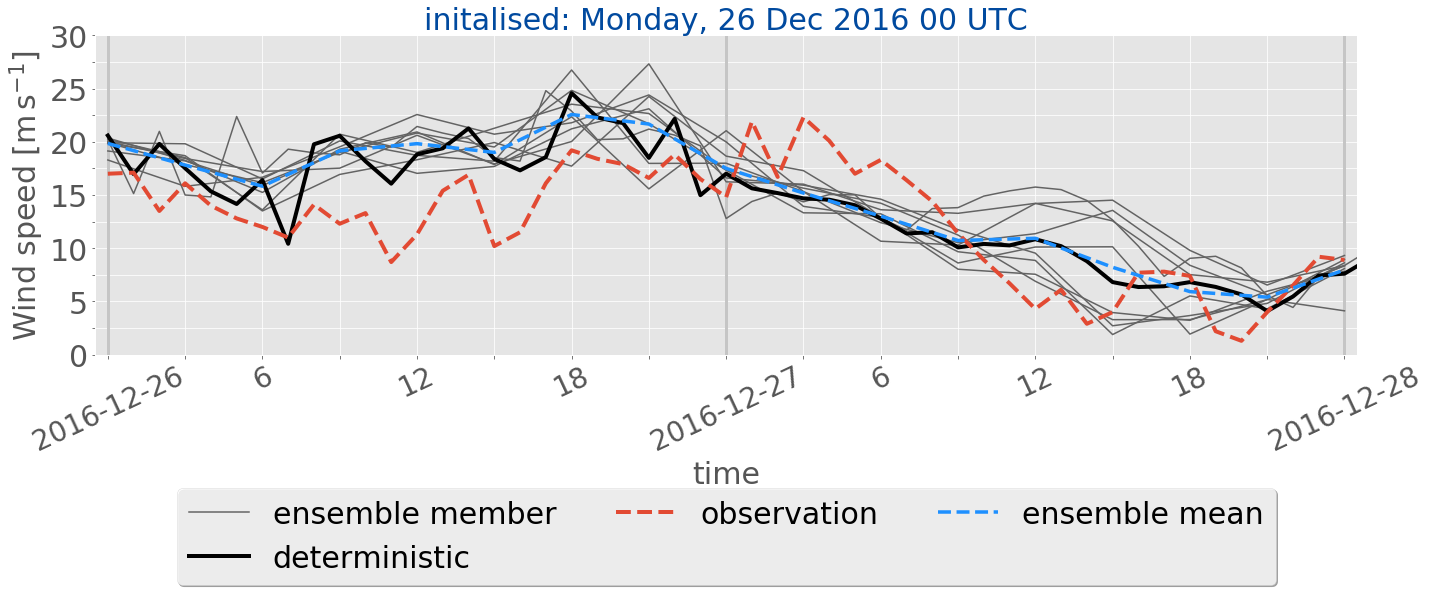
\includegraphics[trim={0.cm 1.5cm 0cm 0cm},clip,
		width=\textwidth]{./fig_sfc_ws/20161226_00}
		\caption{}\label{fig:res:sfc_ws26}
	\end{subfigure}
	
	% sfc precip
	\begin{subfigure}[b]{0.75\textwidth}
		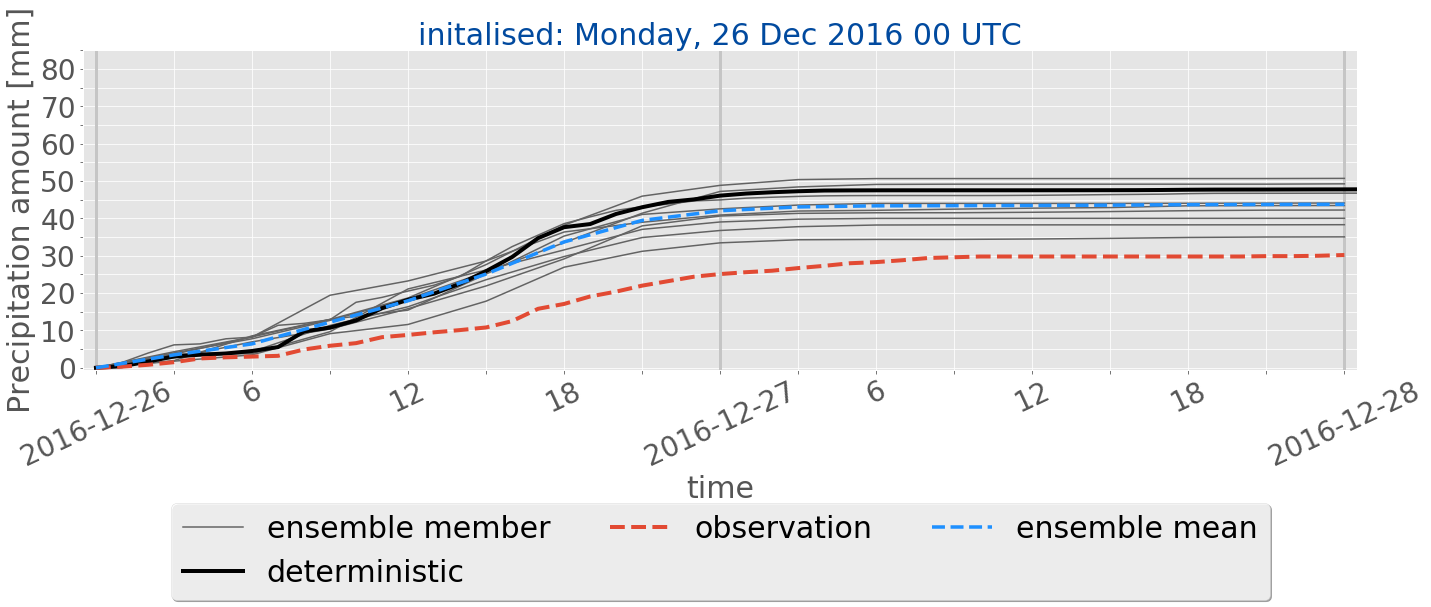
\includegraphics[trim={0.cm 1.5cm 0cm 0cm},clip,
		width=\textwidth]{./fig_sfc_precip/20161226_00}
		\caption{}\label{fig:res:sfc_precip26}
	\end{subfigure}
	% label
	\begin{subfigure}[b]{0.8\textwidth}
		\centering
		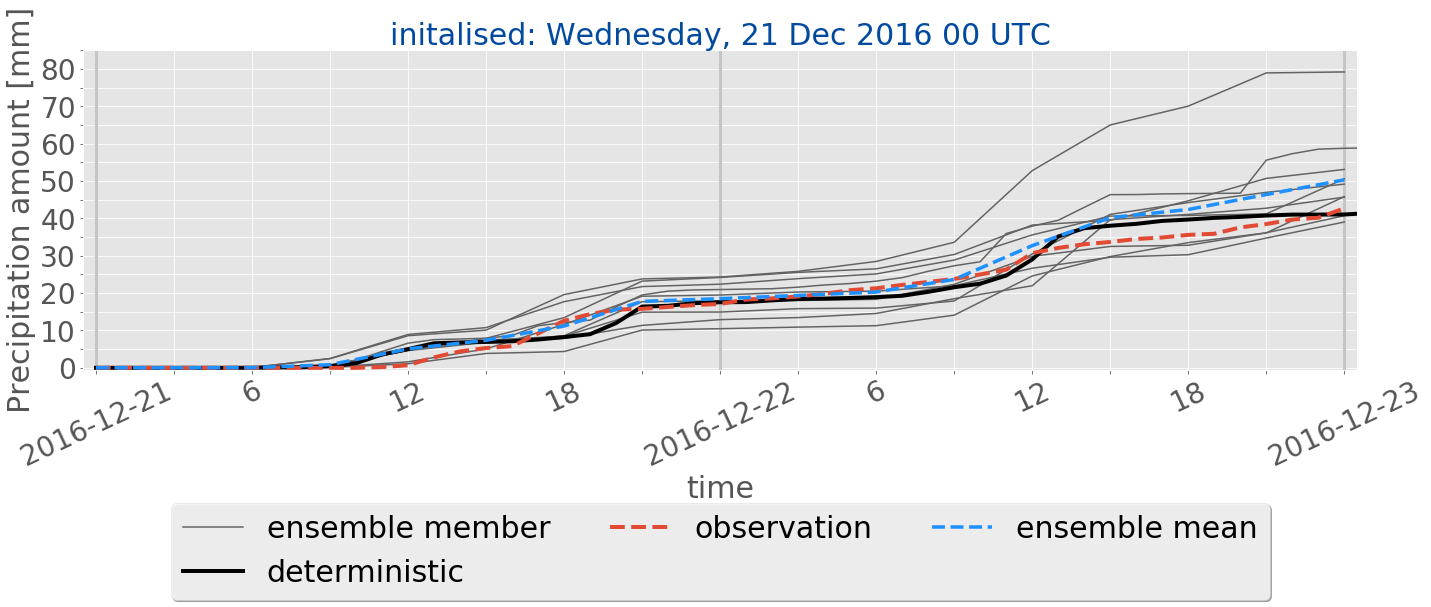
\includegraphics[trim={5.5cm 0cm 5.cm 17.7cm},clip,
		width=0.8\textwidth]{./fig_sfc_precip/20161221_00_label}
	\end{subfigure}
    \caption{\textit{(Continued from previous page.)} Initialisation on \SI{26}{\dec} at \SI{0}{\UTC}.}
\end{figure}
%%%%%%%%%%%%%%%%%%%%%%%%%%%%%%%%%%%%%%%%%%%%%%
\noindent
\\
\textcolor{red}{include R-coefficient}
\Cref{fig:scat:obs_meps} presents the correlation between the observations and the \SI{48}{\hour} MEPS ensemble forecast. The relation for Haukeliseter observations and the MEPS forecast members is indicated with the regression calculated for each day. Sea level pressure has the best correlation of  all variables. The scatter plots in \Cref{fig:scat:obs_meps} show a good correlation for pressure and temperature. Wind direction (\Cref{fig:scat:wd2426}) displays good agreement for \num{24} to \SI{26}{\dec}, but the MEPS forecast imply a disagreement with southerly observed winds in \Cref{fig:scat:wd2123}, between \num{21} and \SI{23}{\dec}. Wind speed is overestimated throughout the event and will be further assessed in \Cref{sec:res:oro_infl} (\Cref{fig:scat:ws2123}, \subref{fig:scat:ws2426}). Surface precipitation amount disagree more between \num{24} and \SI{26}{\dec} than on \num{21} to \SI{23}{\dec} (\Cref{fig:scat:precip2123}, \subref{fig:scat:precip2426}). \Cref{fig:scat:precip2123} suggests a better correlation below \SI{20}{\mm}, for \num{21} to \SI{23}{\dec} than above. A detailed discussion about the precipitation overestimation at the surface is given in \Cref{sec:sfc_acc}.
%%%%%%% image scatter obs ret %%%%%%%%%%%%%%%%
\begin{figure}[t!]
	\centering
	% sfc pressure
	\begin{subfigure}[b]{0.49\textwidth}
		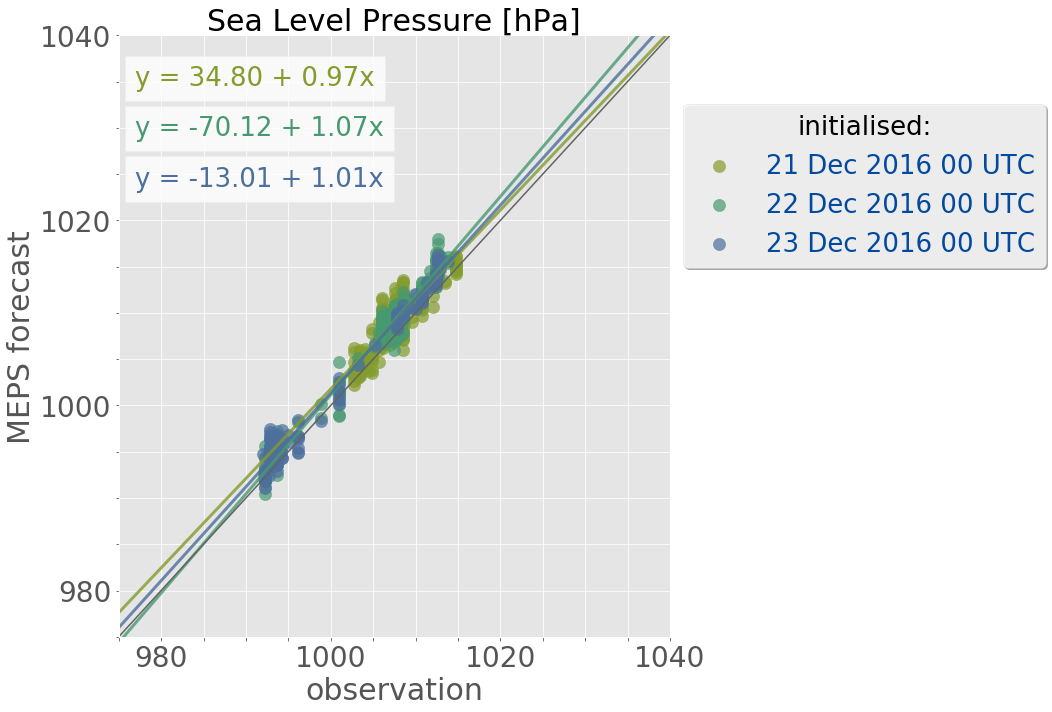
\includegraphics[
		width=\textwidth]{./fig_sfc_pressure/obs_model_20161221_23_00}
		\caption{}\label{fig:scat:pres2123}
	\end{subfigure}
	%
	\begin{subfigure}[b]{0.49\textwidth}
		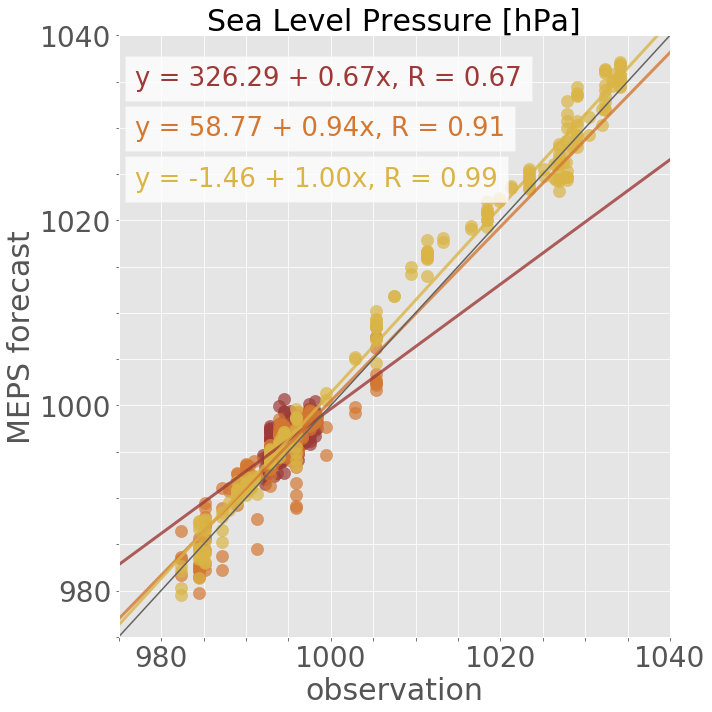
\includegraphics[
		width=\textwidth]{./fig_sfc_pressure/obs_model_20161224_26_00}
		\caption{}\label{fig:scat:pres2426}
	\end{subfigure}
    %
    % label
	\begin{subfigure}[b]{0.49\textwidth}
		\centering
		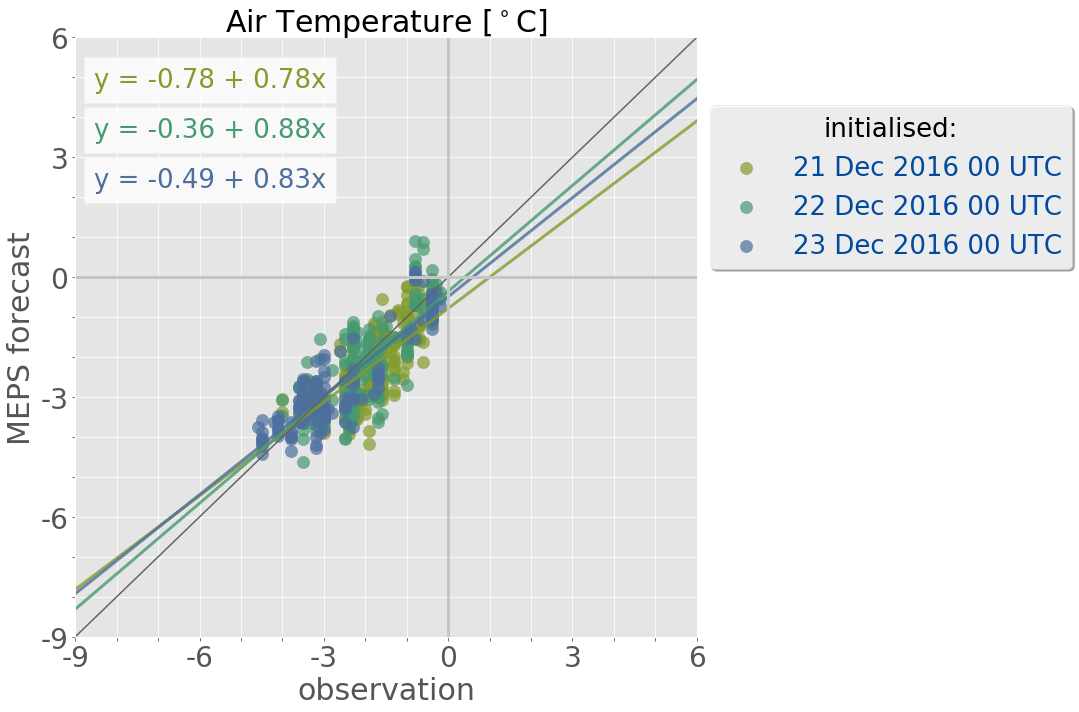
\includegraphics[trim={25.cm 15.5cm 0cm 3.6cm},clip,
		width=0.8\textwidth]{./fig_sfc_temp/obs_model_20161221_23_00_label}
	\end{subfigure}
	\begin{subfigure}[b]{0.49\textwidth}
		\centering
		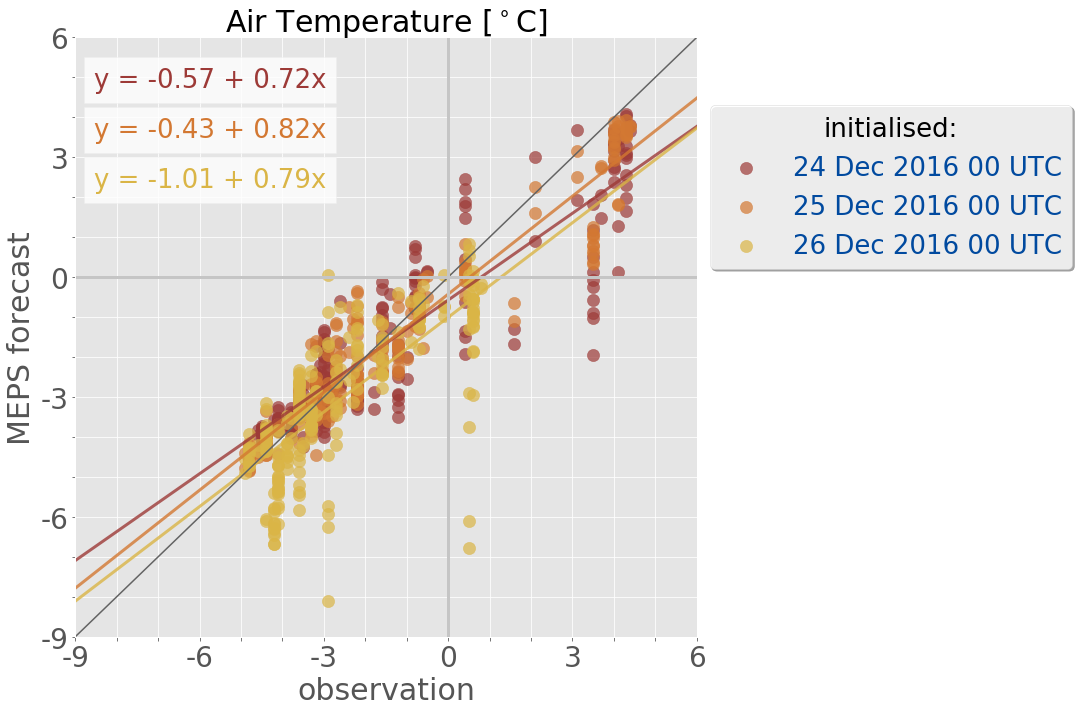
\includegraphics[trim={25.cm 15.5cm 0cm 3.6cm},clip,
		width=0.8\textwidth]{./fig_sfc_temp/obs_model_20161224_26_00_label}
	\end{subfigure}
    \caption{Scatter plots for surface observations and ensemble forecasts initialised for \num{21} to \SI{23}{\dec} (left column, \protect\subref{fig:scat:pres2123}, \protect\subref{fig:scat:temp2123}, \protect\subref{fig:scat:wd2123}, \protect\subref{fig:scat:ws2123}, \protect\subref{fig:scat:precip2123}) and  for \num{24} ton \SI{26}{\dec} (right column, \protect\subref{fig:scat:pres2426}, \protect\subref{fig:scat:temp2426}, \protect\subref{fig:scat:wd2426}, \protect\subref{fig:scat:ws2426}, \protect\subref{fig:scat:precip2426}). The \SI{48}{\hour} scatter values indicate each day, showing the \SIlist{1;3}{\hour} forecasts respectively for \SI{48}{\hour}. \textit{Continued on next page.}  }\label{fig:scat:obs_meps}
\end{figure}
\begin{figure}\ContinuedFloat
	\centering
    %     % sfc temp
	\begin{subfigure}[b]{0.49\textwidth}
		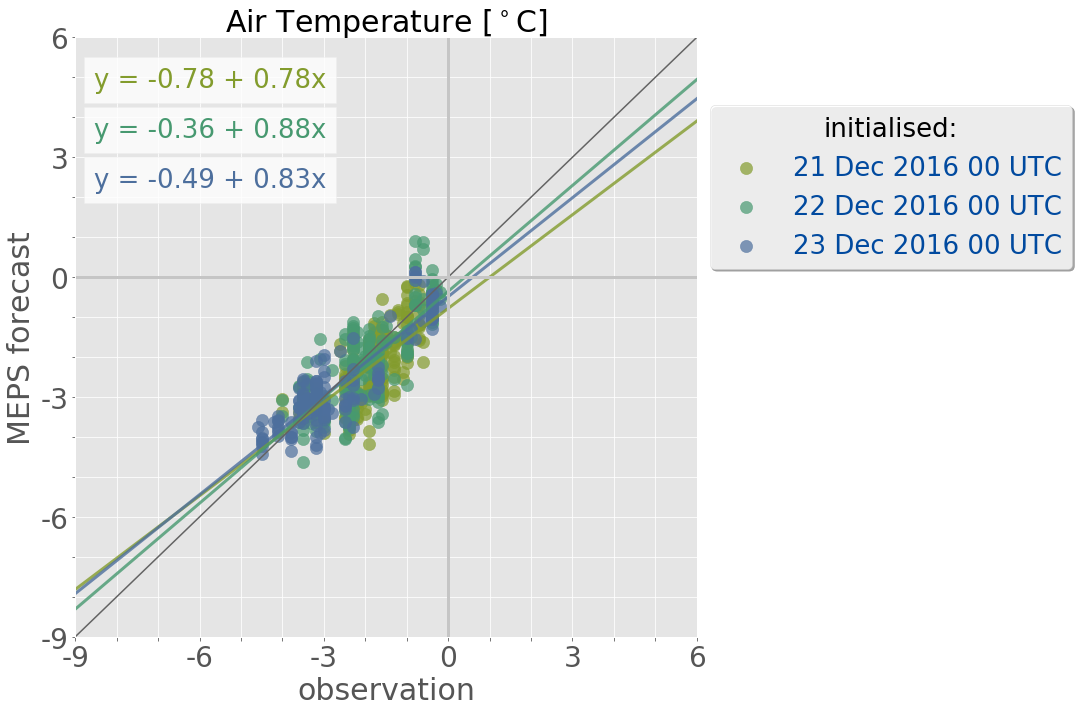
\includegraphics[
		width=\textwidth]{./fig_sfc_temp/obs_model_20161221_23_00}
		\caption{}\label{fig:scat:temp2123}
	\end{subfigure}
	%
	\begin{subfigure}[b]{0.49\textwidth}
		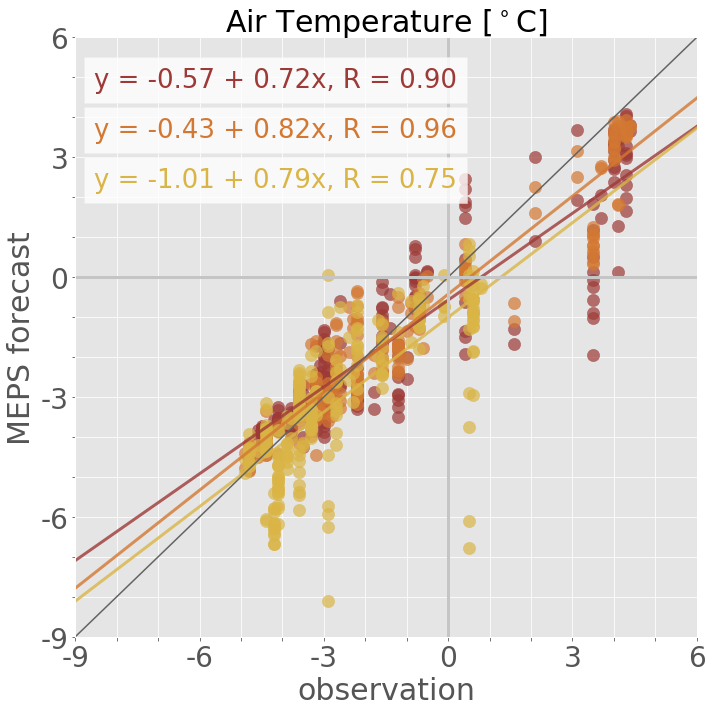
\includegraphics[
		width=\textwidth]{./fig_sfc_temp/obs_model_20161224_26_00}
		\caption{}\label{fig:scat:temp2426}
	\end{subfigure}
% 
	% sfc wd
	\begin{subfigure}[b]{0.49\textwidth}
		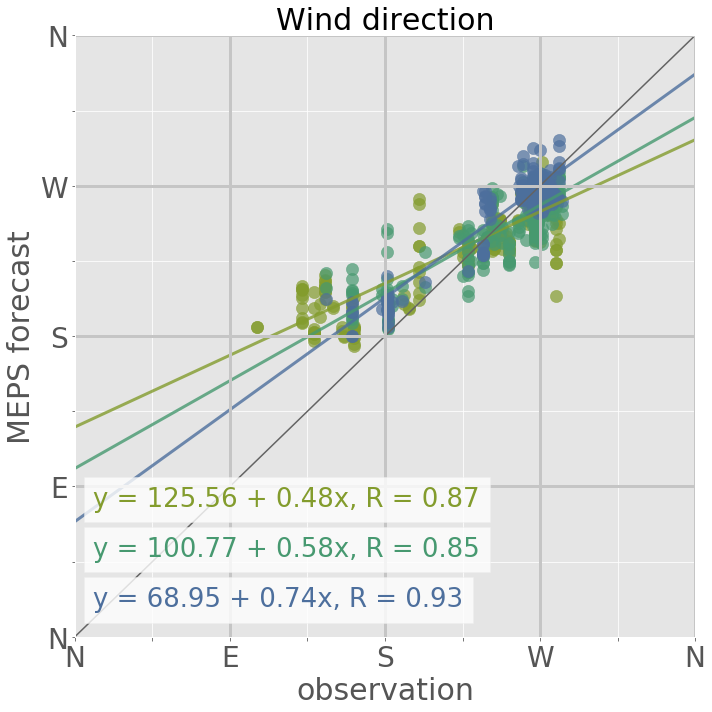
\includegraphics[
		width=\textwidth]{./fig_sfc_wd/obs_model_20161221_23_00}
		\caption{}\label{fig:scat:wd2123}
	\end{subfigure}
	%
	\begin{subfigure}[b]{0.49\textwidth}
		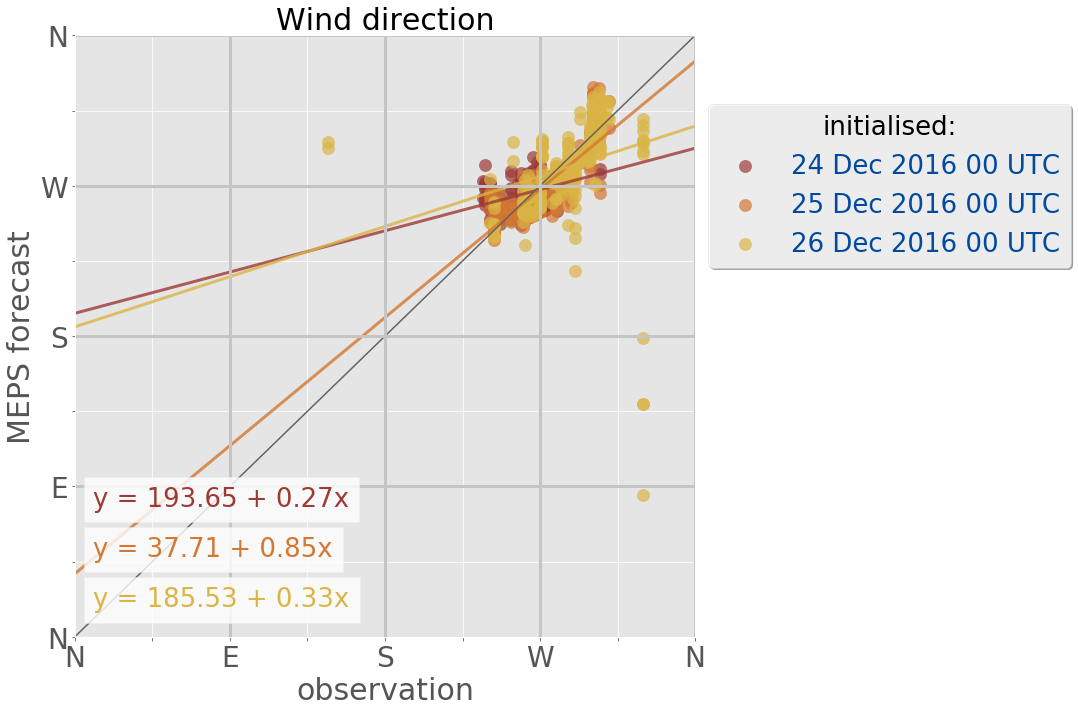
\includegraphics[
		width=\textwidth]{./fig_sfc_wd/obs_model_20161224_26_00}
		\caption{}\label{fig:scat:wd2426}
	\end{subfigure}
    	
	% label
	\begin{subfigure}[b]{0.49\textwidth}
		\centering
		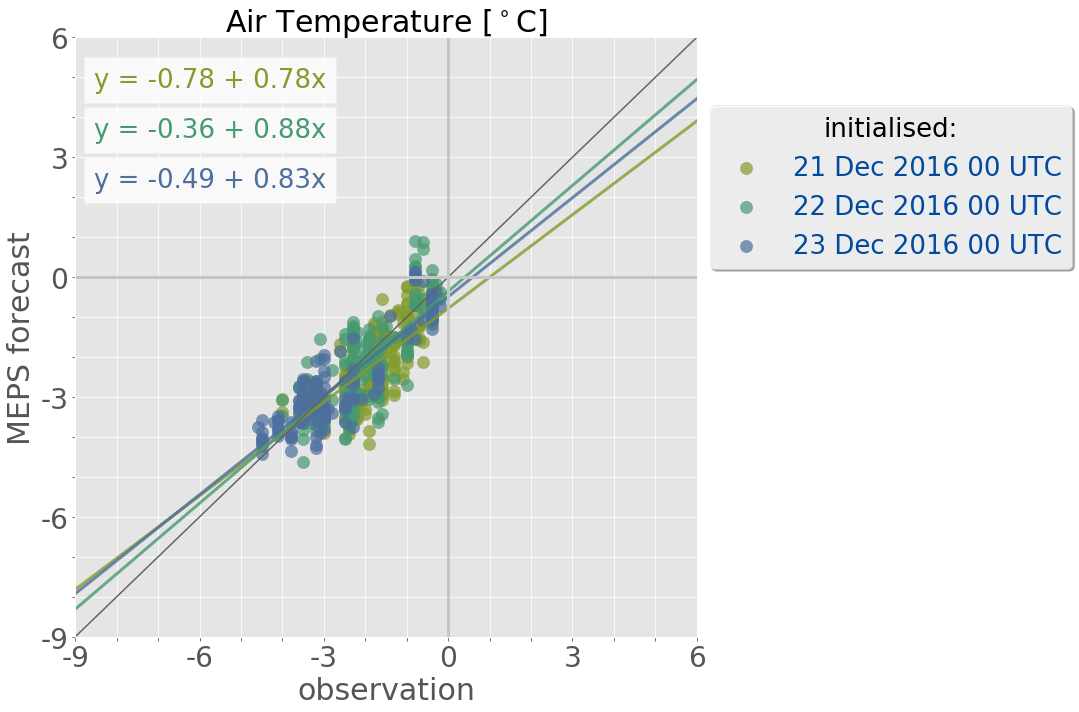
\includegraphics[trim={25.cm 15.5cm 0cm 3.6cm},clip,
		width=0.8\textwidth]{./fig_sfc_temp/obs_model_20161221_23_00_label}
	\end{subfigure}
	\begin{subfigure}[b]{0.49\textwidth}
		\centering
		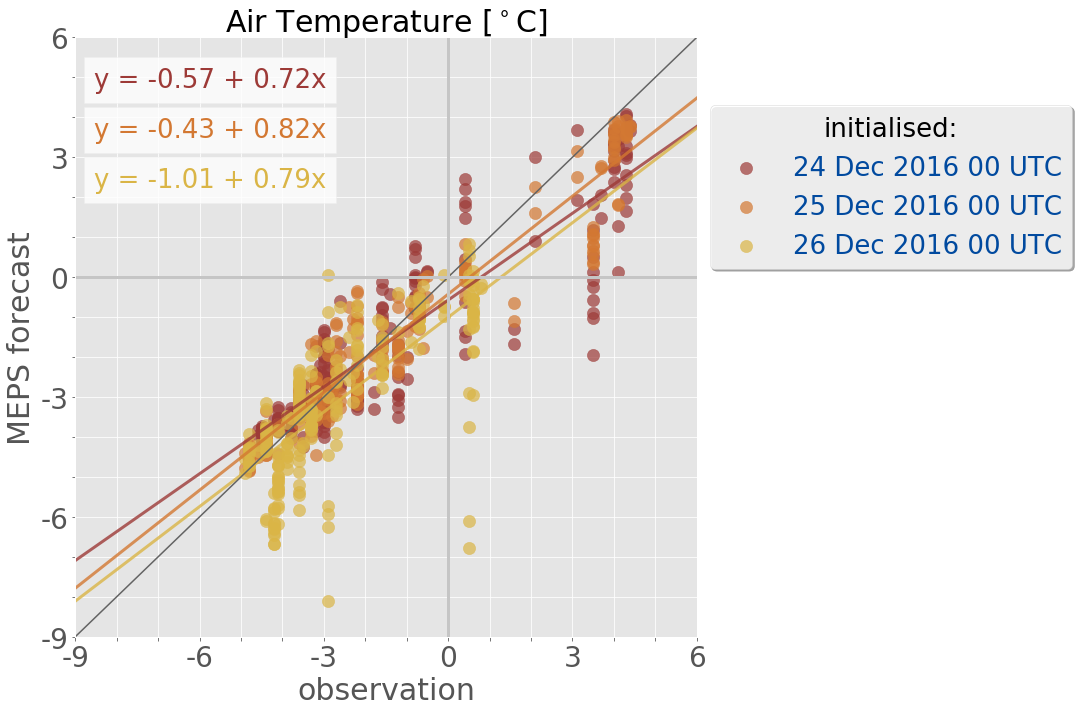
\includegraphics[trim={25.cm 15.5cm 0cm 3.6cm},clip,
		width=0.8\textwidth]{./fig_sfc_temp/obs_model_20161224_26_00_label}
	\end{subfigure}
    \caption{\textit{(Continued from previous page.)} Upper panel \SI{2}{\metre} air temperature, second panel \SI{10}{\metre} wind direction.}
\end{figure}
\begin{figure}\ContinuedFloat
	% sfc ws
	\begin{subfigure}[b]{0.49\textwidth}
		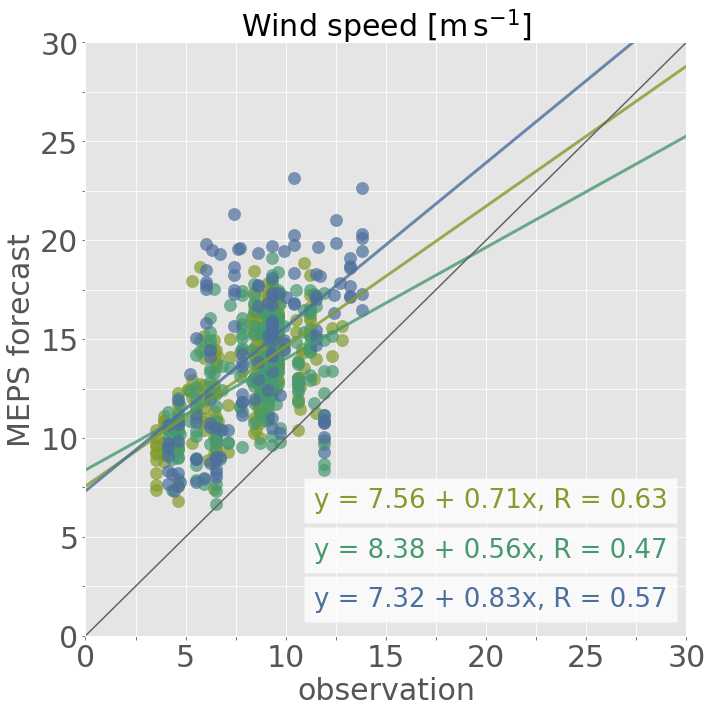
\includegraphics[
		width=\textwidth]{./fig_sfc_ws/obs_model_20161221_23_00}
		\caption{}\label{fig:scat:ws2123}
	\end{subfigure}
	%
	\begin{subfigure}[b]{0.49\textwidth}
		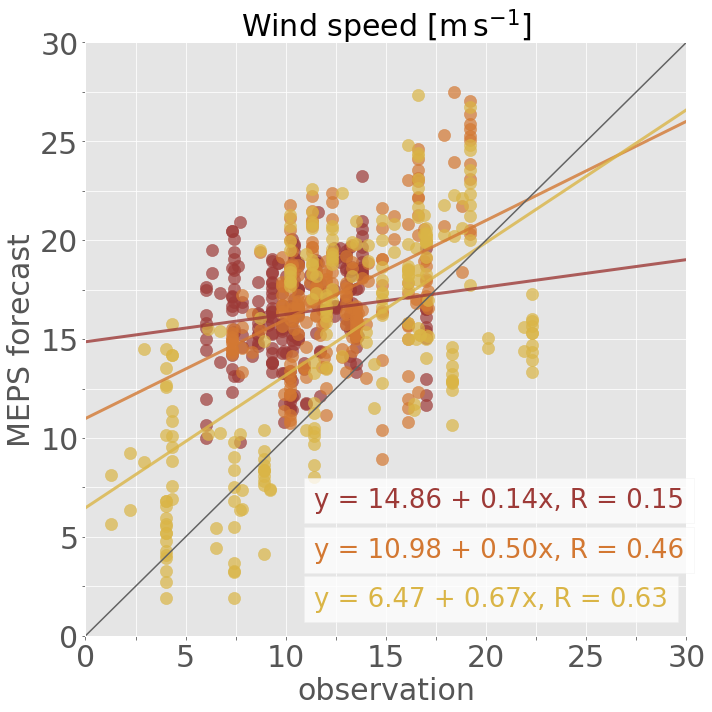
\includegraphics[
		width=\textwidth]{./fig_sfc_ws/obs_model_20161224_26_00}
		\caption{}\label{fig:scat:ws2426}
	\end{subfigure}
	% sfc precip
	\begin{subfigure}[b]{0.49\textwidth}
		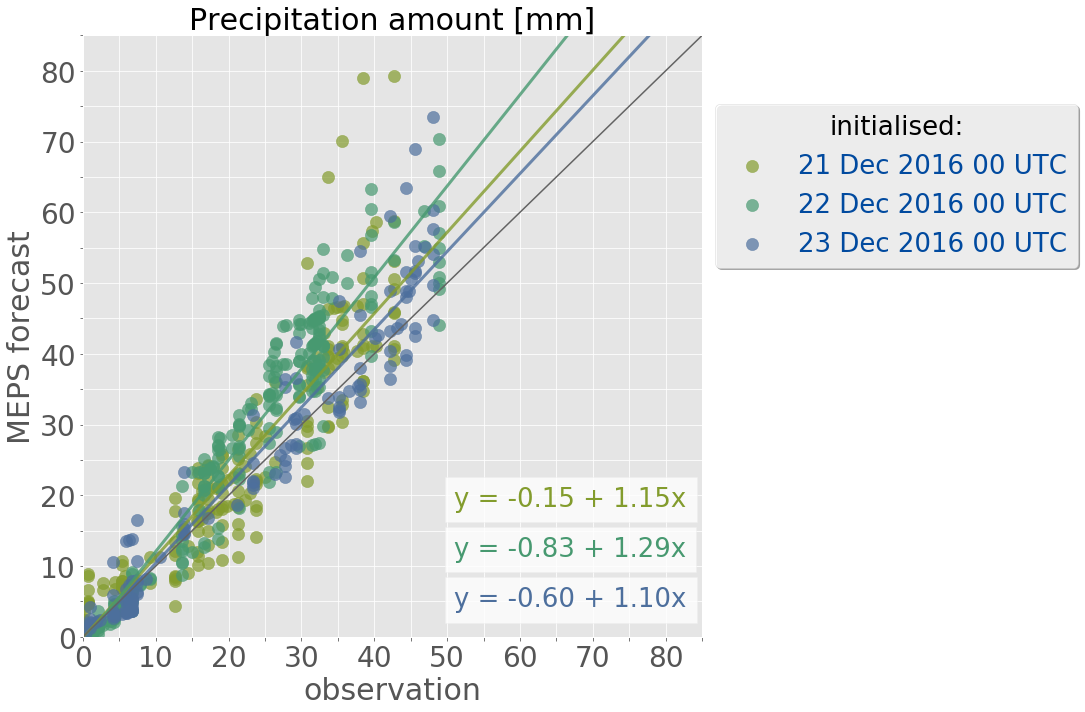
\includegraphics[
		width=\textwidth]{./fig_sfc_precip/obs_model_20161221_23_00}
		\caption{}\label{fig:scat:precip2123}
	\end{subfigure}
	%
	\begin{subfigure}[b]{0.49\textwidth}
		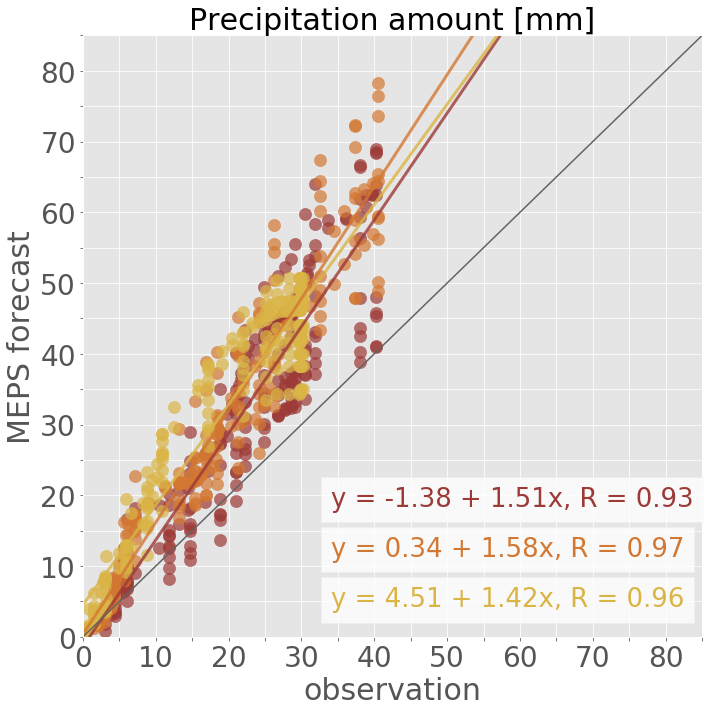
\includegraphics[
		width=\textwidth]{./fig_sfc_precip/obs_model_20161224_26_00}
		\caption{}\label{fig:scat:precip2426}
	\end{subfigure}
	% label
	\begin{subfigure}[b]{0.49\textwidth}
		\centering
		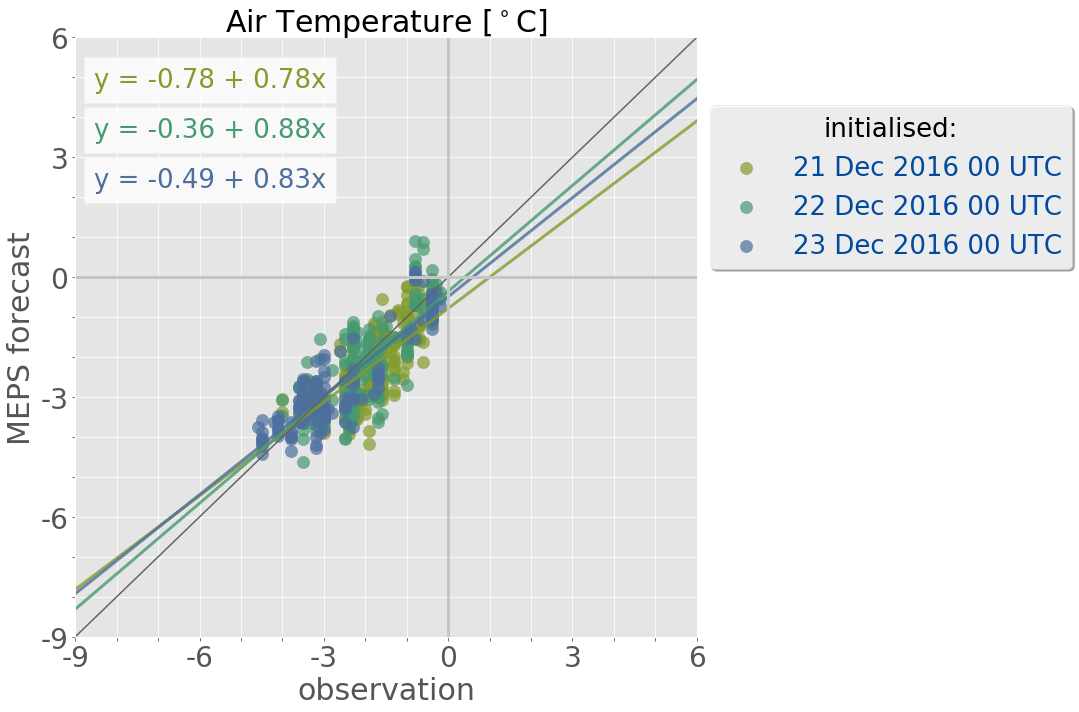
\includegraphics[trim={25.cm 15.5cm 0cm 3.6cm},clip,
		width=0.8\textwidth]{./fig_sfc_temp/obs_model_20161221_23_00_label}
	\end{subfigure}
	\begin{subfigure}[b]{0.49\textwidth}
		\centering
		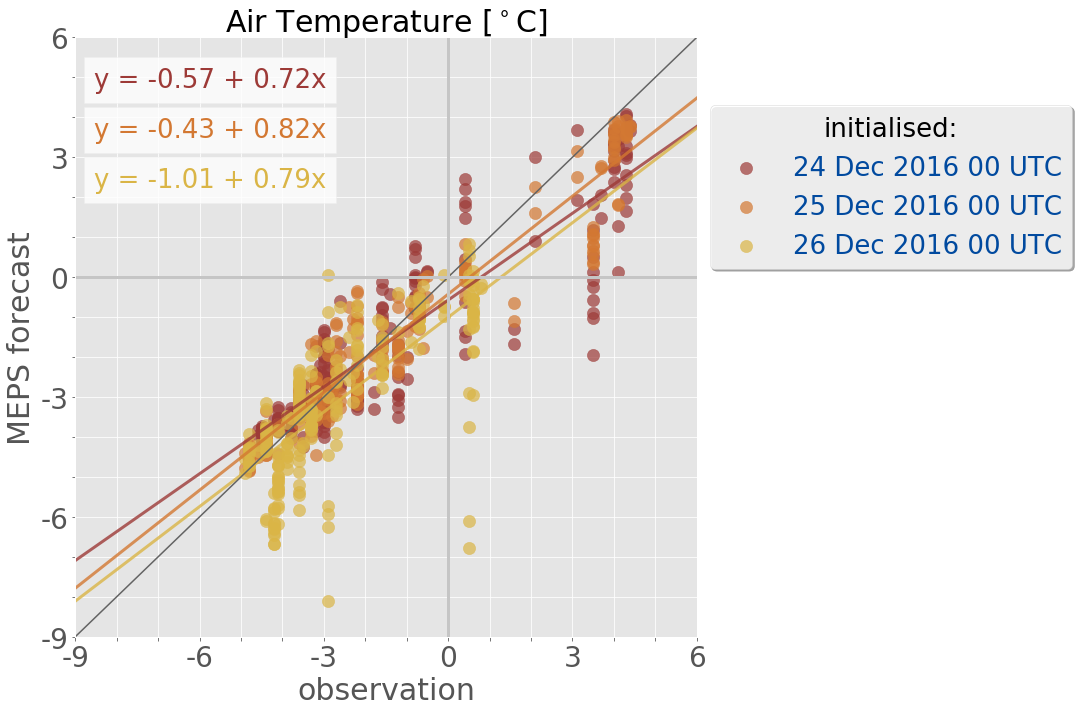
\includegraphics[trim={25.cm 15.5cm 0cm 3.6cm},clip,
		width=0.8\textwidth]{./fig_sfc_temp/obs_model_20161224_26_00_label}
	\end{subfigure}
	\caption{\textit{(Continued from previous page.)} Upper panel \SI{10}{\metre} wind speed, lower panel surface precipitation amount comparing double fence observations to \SI{48}{\hour} MEPS forecasts. }
\end{figure}
%%%%%%%%%%%%%%%%%%%%%%%%%%%%%%%%%%%%%%%%%%%%%%
\noindent
\\
On \num{23} and \SI{26}{\dec}, pressure decreases and increases, as well as temperature increases, and wind changes are present. Since these changes show in the surface observations in \Cref{fig:res:sfc_pres23,fig:res:sfc_temp23,fig:res:sfc_wd23,fig:res:sfc_ws23,fig:res:sfc_precip23} and, \Cref{fig:res:sfc_pres26,fig:res:sfc_temp26,fig:res:sfc_wd26,fig:res:sfc_ws26,fig:res:sfc_precip26}, it is assumed that frontal boundaries passed through Haukelieseter. The \SI{25}{\dec} shows an increase of temperature between \SIlist{15;17}{\UTC} leading to the assumption of a warm air evolution in \Cref{fig:res:sfc_temp25}. The overall weather situation, described in \Cref{sec:largeScale}, showed that a warm front as well as cold front influenced Norway, on \SI{25}{\dec}. Since pressure and wind do not indicate a change related to frontal development, it is assumed that only the warm air section between the warm and cold front is shown in the surface measurements at Haukeliseter (\Cref{fig:res:sfc_temp25}).   
\\
As described in \Cref{sec:largeScale} the ECMWF dynamic tropopause analysis (\Cref{fig:DT23}) shows more ridging at the DT level on \SI{23}{\dec}, than on the previous days. Warm air is advected closer over to Southern Norway (\Cref{fig:DT23}). The low-pressure system approaches in the course of the day south-east of Iceland and hence stronger west to south west wind are associated with the cyclone (\Cref{fig:GP23}). The MEPS forecast, initialised on \SI{23}{\dec} at \SI{0}{\UTC} in \Cref{fig:res:sfc_pres23} follows the observations and shows the decrease in pressure after \SI{12}{\UTC} due to the shift of the occluded front with a constant pressure after the transition. Since warmer air is more advected to the north and the DT in \Cref{fig:DT23} shows a warm low-pressure core, an increase in temperature is observed and predicted at the measurement site (\Cref{fig:res:sfc_temp23}). \textcolor{red}{Include L, H in the surface pressure images}
\\
As the cyclone is advected to the north-east, closer into the Norwegian Sea, a wind change is seen in the ECMWF analysis (\Cref{fig:GP23}). First west wind and later south-west wind is associated with the low-pressure system. The MEPS forecast and observations in \Cref{fig:res:sfc_wd23} and \subref{fig:res:sfc_ws23} indicate a wind change from west to south with a slight decrease in wind speed.
\\
On \SI{23}{\dec}, the evolution of the occlusion is also observed by an increase in precipitation. Before \SI{18}{\UTC} the surface accumulation shows light precipitation (\Cref{fig:res:sfc_precip23}). During the passage of the occlusion, the observed surface accumulation increases which is associated to continuous, heavy precipitation shown in \Cref{fig:res:sfc_precip23}.
\\
\\
Similar patterns as on \SI{23}{\dec} were seen for the evolution of the occluded front on \SI{26}{\dec} in the ECMWF analysis \Cref{fig:DT26} and \ref{fig:GP26}. In this case the low-pressure system was located north of Møro and Romsdal in the Norwegian Sea. In the morning the cyclone is located east of Iceland and in the course of the day it moves closer to the coast of Norway (\Cref{fig:DT26_18} and \ref{fig:GP26_18}). Before landfall at \SI{16}{\UTC}, a pressure decrease occurs at Haukeliseter (\Cref{fig:res:sfc_pres26}). During the development of the occluded front, the sea level pressure reaches its lowest point of \SI{985}{\hPa} (\Cref{fig:res:sfc_pres26}) and increases afterwards during the dissipation of the 2016 Christmas storm. 
%% Pressure, temperature, and wind changes for the occlusion transition were already forecasted for initialisations on \SI{25}{\dec} (\Cref{fig:res:sfc_pres25}, \subref{fig:res:sfc_temp25}, \subref{fig:res:sfc_wd25}, \subref{fig:res:sfc_ws25}), only wind speed and precipitation seem not to agree with the observations at Haukeliseter. 
\\
Since the cyclone was surrounded by colder air (south of the low-pressure system in \Cref{fig:DT26}), first a drop and then an increase of temperature were observed and forecasted by MEPS (\Cref{fig:res:sfc_temp26}). An indication of the occlusion evolution is also visible in the \SI{10}{\metre} wind observations and MEPS predictions in \Cref{fig:res:sfc_wd26} and \subref{fig:res:sfc_ws26}. 
On \SI{26}{\dec} at \SI{0}{\UTC}, the low pressure system is east of Iceland (not shown), moving closer into the Norwegian Sea by \SI{12}{\UTC} (\Cref{fig:DT26} and \ref{fig:GP26}). 
Surface west winds are associated to the cyclone in the Norwegian Sea, and impinging on the West coast of Norway \Cref{fig:GP26}. The wind measurement and MEPS forecast in \Cref{fig:res:sfc_wd26} and \ref{fig:res:sfc_ws26}, show a gentle west breeze of up to \SI{17}{\mPs} at Haukeliseter before \SI{12}{\UTC}.
The centre of the occluded front is located over Norway at \SI{18}{\UTC}, and the pronounced surface pressure gradient, in \Cref{fig:GP26_18}, indicate an increase in surface wind with a north-west wind direction. During this transition of the occlusion, the wind direction changes to north-west with higher observed wind speeds up to \SI{20}{\mPs} (\Cref{fig:res:sfc_wd26} and \ref{fig:res:sfc_ws26}). 
\\
Precipitation is continuing throughout the day, with light to moderate precipitation before the occlusion passage seen in \Cref{fig:res:sfc_precip26}. Heavy precipitation related to the occlusion, around \SI{16}{\UTC}, is followed by moderate to light deposition on \SI{26}{\dec}. 
\\
%%%%%%% image liquid obs particle %%%%%%%%%%%%%%%%
\begin{figure}[t]
	\centering
	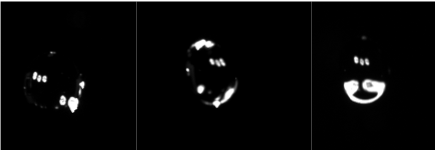
\includegraphics[%trim={45.cm 30.cm 13cm 35cm},clip,
	width=0.8\textwidth]{./MASC_obs/Masc_obs_liquid_2512}
	\caption{MASC images of falling water drops observed on \SI{25}{\dec} at \SI{17}{\UTC} from three different angles. Not all parts of the liquid sphere are equally illuminated.}\label{fig:res:obs_masc}
\end{figure}
%%%%%%%%%%%%%%%%%%%%%%%%%%%%%%%%%%%%%%%%%%%%%%
\\
While on \num{23} and \SI{26}{\dec} precipitation was associated with a transition respectively landfall of an occlusion, the \SI{25}{\dec} was marked by the transition of a warm sector. The ECMWF analysis shows a ridging of warm air at the dynamic tropopause (\Cref{fig:DT25}). The cyclone core is south east of Iceland in \Cref{fig:DT25} with two associated frontal boundaries. While the warm front is approaching the west coast, the cold front is north-west of Great Britain. In \Cref{fig:GP25}, the tail of the cold front moved into lower latitudes, following the slowdown of front, leading to a stationary frontal boundary. Furthermore, the mid-latitude jet is aligned with the surface frontal boundaries (\Cref{fig:DT25_00}), while the Haukeliseter site is located below the the midlatitudal jet (\Cref{fig:GP25_00}). %This leads to rising motion at the surface.
\\
Neither pressure nor wind observations and forecasts in \Cref{fig:res:sfc_pres25}, \subref{fig:res:sfc_wd25}, and \subref{fig:res:sfc_ws25}, indicate the evolution of any frontal boundary. The only indication of a transition could be seen in the increase and then decrease of temperature at \SI{11}{\UTC} until \SI{21}{\UTC} (\Cref{fig:res:sfc_temp25}). In \Cref{fig:res:sfc_wd25}, a small wind change from west to north-west is observed by the wind mast at \SI{10}{\UTC}, which is not forecasted by MEPS, it rather estimated strong westerly winds.
\\
Particle images taken by the MASC are available on \SI{25}{\dec}, during the transition of the warm sector in \Cref{fig:res:obs_masc}. Without theses images taken around \SI{17}{\UTC} it would only be possible to verify that liquid precipitation occurred with the optical precipiation detectors at the Haukeliseter site. Together with the increase in surface temperature (\Cref{fig:res:sfc_temp25}) it can be concluded that the warm sector of the Christmas 2016 event passed by the measurement site.
\textcolor{red}{KICKI: Should I include the DIANA analysis maps? But the meteorologist also use ECMWF to make them!}
%
\\
\\
The comparison between the ECMWF analysis (\Cref{sec:largeScale}) and the observations at the measurement site (\Cref{fig:res:sfc_obs_meps}), led conclude that the ensemble member forecast system MEPS covers the prediction of large scale phenomena like occlusions and fronts, as well as liquid precipitation at the surface. 
\\
The scatter plots for observations and MEPS forecast show good correlation for most variables (\Cref{fig:scat:pres2123,fig:scat:pres2426,fig:scat:temp2123,fig:scat:temp2426}, and \subref{fig:scat:wd2426}).
The best agreement for pressure is reached on \SI{26}{\dec} (\Cref{fig:res:sfc_pres26}), when the Christmas storm hit land and dissipated after the evolution of the occlusion at \SI{16}{\UTC}. \citet{dahlgren_comparison_2013} showed an improvement of sea level pressure forecast for AROME, by including large scale boundary conditions for ECMWF into the regional model. The observation-model comparison by \citet{dahlgren_comparison_2013} showed a decrease of pressure bias with lead time after \SI{24}{\hour} with the use of pressure mixing. 
Since surface pressure is in good agreement with the observations, it is assumed that the warm front did not pass through Haukeliseter on \SI{25}{\dec} and only the warm sector associated with the 2016 Christmas storm is observed. This shows a quite detailed forecast ability of MEPS, as from the ECMWF analysis, in \Cref{fig:DT25}, it is not quite clear if the warm front could have passed through. To be sure that the warm front did not pass through Haukeliseter, or whether it is a predictive error of MEPS, surface pressure, temperature and wind should be compared to the nearest grid point of the global forecast model ECMWF to verify this result.
\\
\Cref{fig:scat:temp2426} displays a moderate correlation between observation and the \SI{48}{\hour} MEPS ensemble member forecast system. In general, MEPS underestimates the observed \SI{2}{\metre} air temperature, but MEPS estimated the surface temperature changes at the correct occurrence for \num{23}, \num{25}, and \SI{26}{\dec}. 
\\
\Cref{fig:bias:temp} shows warm and cold biases for \num{23} and \SI{26}{\dec}, respectively. On \SI{25}{\dec}, within the warm sector a cold bias was observed, underestimating the temperature when compared to the observation.  The forecasts for \num{23}, \num{25}, and \SI{26}{\dec} show calculated mean absolute error values (\Cref{eq:MAE}) of up to \SIlist{0.61;0.77;1.44}{\kelvin} in \Cref{fig:MAE:temp}. 
The previous operational deterministic forecast model AROME-MetCoOp showed a cold bias of \SI{2}{\metre} temperature for the Norwegian mean, during winter 2013 with the introduction of AROME-Norway and later AROME-MetCoOp \citep{muller_arome-metcoop:_2017}. 
The mean error for the Norwegian model domain of AROME-MetCoOP estimated by \citet{muller_arome-metcoop:_2017} is smaller than \SI{1.8}{\kelvin} for the surface \SI{2}{\metre} temperature in December 2014. 
The new ensemble forecast system MEPS shows a reduction of mean errors for the Christmas 2016 extreme event, when compared to the Norwegian mean of AROME-MetCoOp.
%%% image bias %%%%%%%%%%%%%%%%%%%%%%%%%%%%%%%%%%%%%
\begin{figure}[H]%\ContinuedFloat
		\centering
        % pres
		\begin{subfigure}[b]{0.8\textwidth}
			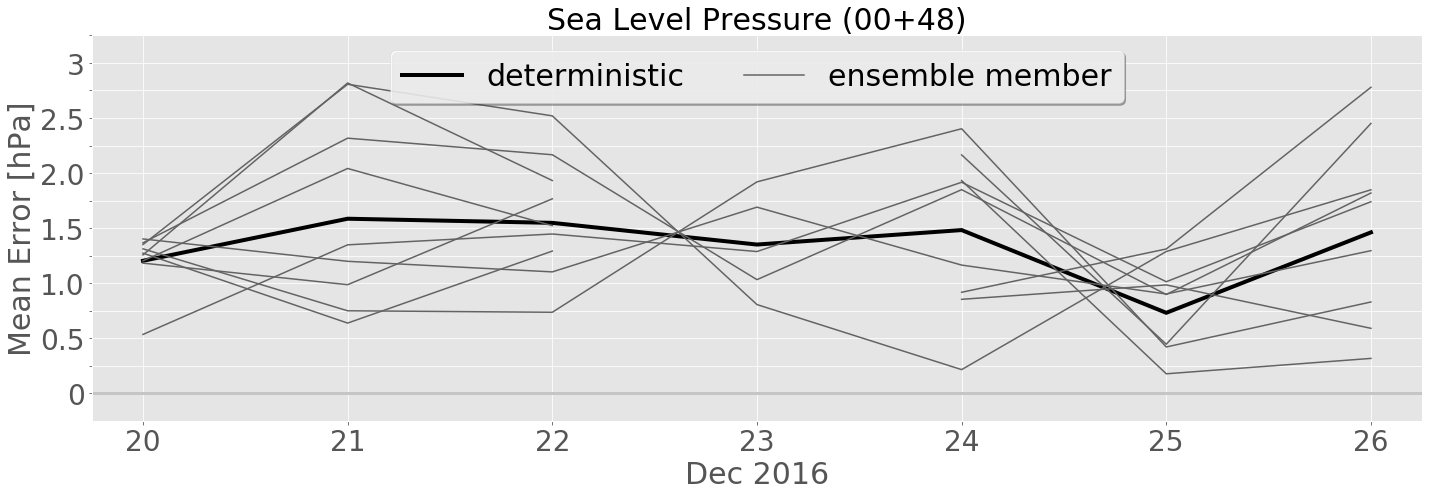
\includegraphics[trim={0cm 0cm 0cm 9.5cm},clip,width=\textwidth]{./fig_sfc_pressure/ME_20161220_26_00}
			\caption{}\label{fig:bias:pres}
		\end{subfigure}
        % temp
		\begin{subfigure}[b]{0.8\textwidth}
			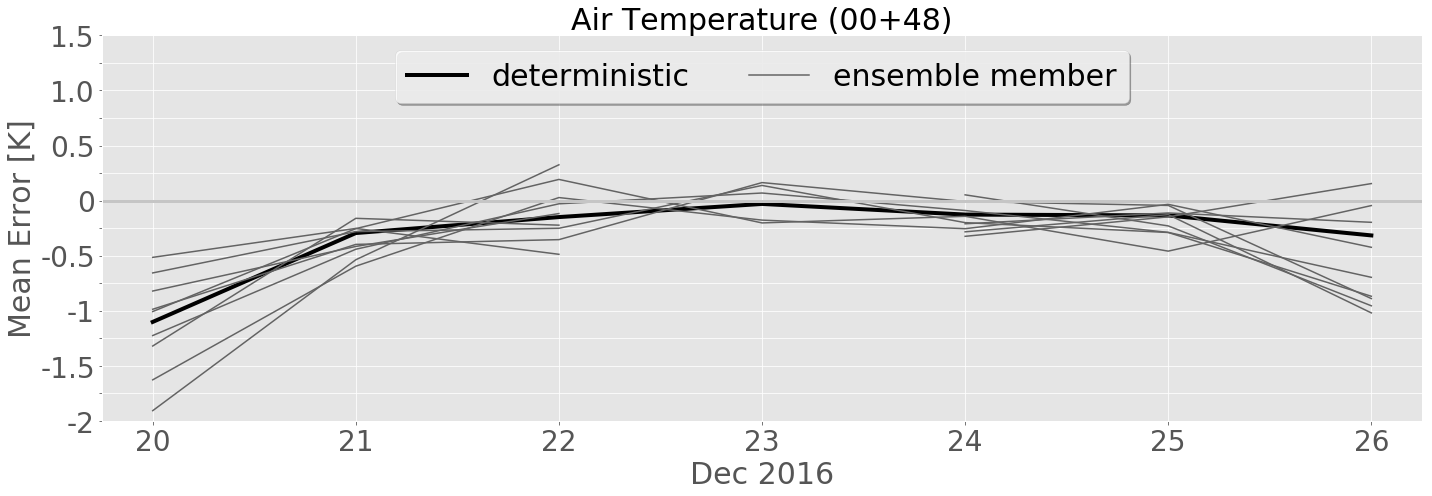
\includegraphics[trim={0cm 0cm 0cm 9.5cm},clip,width=\textwidth]{./fig_sfc_temp/ME_20161220_26_00}
			\caption{}\label{fig:bias:temp}
		\end{subfigure}
        % wd
		\begin{subfigure}[b]{0.8\textwidth}
			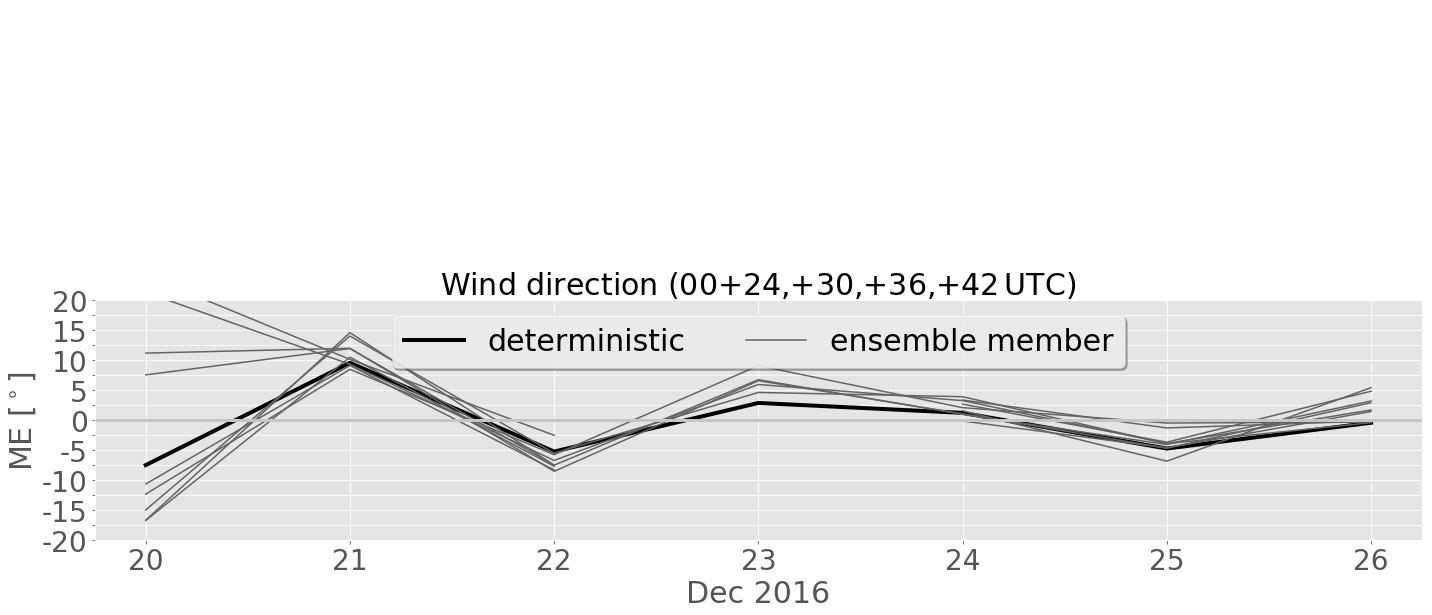
\includegraphics[trim={0cm 0cm 0cm 9.5cm},clip,width=\textwidth]{./fig_sfc_wd/ME_20161220_26_00}
			\caption{}\label{fig:bias:wd}
		\end{subfigure}
% \end{figure}
% \begin{figure}\ContinuedFloat
	\centering
		% ws
		\begin{subfigure}[b]{0.8\textwidth}
			\includegraphics[trim={0cm 0cm 0cm 9.5cm},clip,width=\textwidth]{./fig_sfc_ws/ME_20161220_26_00}
			\caption{}\label{fig:bias:ws}
		\end{subfigure}
% \end{figure}
% \begin{figure}\ContinuedFloat
% \centering
%         % precip
% 		\begin{subfigure}[b]{0.75\textwidth}
% 			\includegraphics[width=\textwidth]{./fig_sfc_precip/ME_20161220_26_00}
% 			\caption{}\label{fig:bias:precip}
% 		\end{subfigure}
        % precip 12h
        \begin{subfigure}[b]{0.8\textwidth}
			\includegraphics[trim={0cm 0cm 0cm 9.5cm},clip,width=\textwidth]{./fig_sfc_precip/ME12_20161220_26_00}
			\caption{}\label{fig:bias:precip12}
		\end{subfigure}
	\caption{{Mean error (\protect\subref{fig:bias:pres}, \protect\subref{fig:bias:temp}, \protect\subref{fig:bias:wd}, \protect\subref{fig:bias:ws}, \protect\subref{fig:bias:precip12}) of surface variables for all ten ensemble members at Haukeliseter, initialisations at \SI{0}{\UTC}, valid for \SI{48}{\hour}. From top to bottom, sea level pressure (\protect\subref{fig:bias:pres}), \SI{2}{\metre} air temperature (\protect\subref{fig:bias:temp}), \SI{10}{\metre} wind direction (\protect\subref{fig:bias:wd})},  \SI{10}{\metre} wind speed (\protect\subref{fig:bias:ws}), precipitation accumulation for 
    %\SI{48}{\hour} (\protect\subref{fig:bias:precip}) and 
    \SI{12}{\hour} surface accumulation (\protect\subref{fig:bias:precip12}). } \label{fig:bias} 
\end{figure}
\begin{figure}[H]%\ContinuedFloat
		\centering
        % pres
        \begin{subfigure}[b]{0.8\textwidth}
			\includegraphics[trim={0cm 0cm 0cm 9.5cm},clip,width=\textwidth]{./fig_sfc_pressure/MAE_20161220_26_00}
			\caption{}\label{fig:MAE:pres}
		\end{subfigure}
		% temp
        \begin{subfigure}[b]{0.8\textwidth}
			\includegraphics[trim={0cm 0cm 0cm 9.5cm},clip,width=\textwidth]{./fig_sfc_temp/MAE_20161220_26_00}
			\caption{}\label{fig:MAE:temp}
		\end{subfigure}
        % wd
        \begin{subfigure}[b]{0.75\textwidth}
			\includegraphics[trim={0cm 0cm 0cm 9.5cm},clip,width=\textwidth]{./fig_sfc_wd/MAE_20161220_26_00}
			\caption{}\label{fig:MAE:wd}
		\end{subfigure}
% \end{figure}
% \begin{figure}\ContinuedFloat
	\centering
		% ws
        \begin{subfigure}[b]{0.8\textwidth}
			\includegraphics[trim={0cm 0cm 0cm 9.5cm},clip,width=\textwidth]{./fig_sfc_ws/MAE_20161220_26_00}
			\caption{}\label{fig:MAE:ws}
		\end{subfigure}
% \end{figure}
% \begin{figure}\ContinuedFloat
% \centering
%         % precip
%         \begin{subfigure}[b]{0.75\textwidth}
% 			\includegraphics[width=\textwidth]{./fig_sfc_precip/MAE_20161220_26_00}
% 			\caption{}\label{fig:MAE:precip}
% 		\end{subfigure}
        % precip 12h
        \begin{subfigure}[b]{0.8\textwidth}
			\includegraphics[trim={0cm 0cm 0cm 9.5cm},clip,width=\textwidth]{./fig_sfc_precip/MAE12_20161220_26_00}
			\caption{}\label{fig:MAE:precip12}
		\end{subfigure}
	\caption{Mean absolute error (\protect\subref{fig:MAE:pres}, \protect\subref{fig:MAE:temp}, \protect\subref{fig:MAE:wd}, \protect\subref{fig:MAE:ws}, \protect\subref{fig:MAE:precip12}) of surface variables for all ten ensemble members at Haukeliseter, initialisations at \SI{0}{\UTC}, valid for \SI{48}{\hour}. From top to bottom, sea level pressure (\protect\subref{fig:MAE:pres}), \SI{2}{\metre} air temperature (\protect\subref{fig:MAE:temp}), \SI{10}{\metre} wind direction (\protect\subref{fig:MAE:wd}), \SI{10}{\metre} wind speed (\protect\subref{fig:MAE:ws}), precipitation accumulation for \SI{12}{\hour} surface accumulation (\protect\subref{fig:MAE:precip12}).}\label{fig:MAE}
\end{figure}
%%%%%%%%%%%%%%%%%%%%%%%%%%%%%%%%%%%%%%%%%%%%%%%%%%%%%%%%%%%%%%%%%%%%%%%%%%
\noindent
\\
During the Christmas storm 2016, high wind speeds were observed at the Haukeliseter site (\Cref{fig:res:sfc_ws23}, \subref{fig:res:sfc_ws25}  and \subref{fig:res:sfc_ws26}).
According to \citet{muller_arome-metcoop:_2017} high wind speeds are significantly better simulated for AROME-MetCoOp compared to ECMWF's forecast for the model domain. Wind speed MEPS predictions in \Cref{fig:res:sfc_ws23}, \subref{fig:res:sfc_ws25}, and \subref{fig:res:sfc_ws26} displays still an overestimation of wind speeds throughout the event. Furthermore, the correlation of observations and wind speed in \Cref{fig:scat:ws2123} and \subref{fig:scat:ws2426} show an overestimation for stronger wind speeds on \num{24} to \SI{26}{\dec} than for \num{21} to \SI{23}{\dec}. 
The mean absolute error for wind speed during the Christmas storm is ranging from \SIrange{3}{7}{\mPs} for \SI{48}{\hour} lead time.
During the three days of frontal transitions, the highest mean absolute error of \SI{6.5}{\mPs} occurs for initialisations on \SI{23}{\dec}.
The inaccuracy for wind speeds is an already known difficulty in the deterministic version of MEPS \citep{muller_arome-metcoop:_2017}. \citet{muller_arome-metcoop:_2017} presented, that AROME-MetCoOp wind speed prediction generally agreed better with observations for wind speeds between \SIrange{3}{13}{\mPs} than ECMWF forecasts did, showing the advantage of a high-resolution weather model. Furthermore, with increasing wind speed the forecast accuracy for the Norwegian mean decreased with a mean absolute error below \SI{2}{\mPs} for \SIrange{6}{24}{\hour} lead times, in December 2014 in AROME-MetCoOp. \citet{muller_arome-metcoop:_2017} study case showed a slight underestimation of ECMWF \SI{10}{\metre} wind compared to the Norwegian AROME-MetCoOp forecast for February 2015.%, but still overestimates MEPS the wind.
On \SI{23}{\dec}, the mean absolute error is more than three times as high as the monthly averaged value for the Norwegian forecast domain (\SI{2}{\mPs} for \SIrange{6}{24}{\hour} forecast time) from \citet{muller_arome-metcoop:_2017}. The larger mean absolute error during the event is firstly related to the comparison of a long term study of \citet{muller_arome-metcoop:_2017}, secondly their mean absolute error monthly average for \SIrange{6}{24}{\hour} lead times, and third to the location of Haukeliester. 
\\
Haukeliseter is a measurement site exposed to high wind speeds \citep{wolff_measurements_2013,wolff_derivation_2015}. The ensemble prediction system MEPS seems to still have issues forecasting the wind speed correctly in mountainous terrain.
A detailed insight to the orographical wind influence will be assessed in \Cref{sec:res:oro_infl}. 
\\
Pressure, temperature, and wind changes for the occlusion transition on \SI{26}{\dec} were already forecasted for initialisations on \SI{25}{\dec} (\Cref{fig:res:sfc_pres25}, \subref{fig:res:sfc_temp25}, \subref{fig:res:sfc_wd25}, \subref{fig:res:sfc_ws25}), only wind speed and precipitation seem not to agree with the observations at Haukeliseter. The same is true for \SI{25}{\dec}, when the warm sector passes through Haukeliseter. 
\\
\Cref{fig:res:sfc_precip21}, \subref{fig:res:sfc_precip23}, \subref{fig:res:sfc_precip25}, and \subref{fig:res:sfc_precip26} illustrate the surface precipitation amount observed and predicted by MEPS for Haukeliseter. MEPS overestimation is shown for precipitation when the cyclone intensifies and gets closer to Norway on \num{24}, \num{25} and \SI{26}{\dec}. The surface observations and MEPS predictions in \Cref{fig:scat:precip2123} and \subref{fig:scat:precip2426} show an overestimate for \num{24}, \num{25} and \SI{26}{\dec}, whereas on \num{21}, \num{22}, and \SI{23}{\dec} the surface accumulation is balanced for  predictions up to \SI{30}{\mm}. Any reasons for the overestimation of precipitation accumulation on the ground will be further analysed and discussed in \Cref{sec:sfc_acc}. 
\textcolor{red}{What could be still a weakness that the model overestimates the wind speed? In \citet{muller_arome-metcoop:_2017}: change from ECOCLIMAP1 because the surface roughness was too low and followed high wind speeds? Is this still the case for MEPS? High wind speeds followed also from wrongly adressed 'permanent snow'. Do not use 'orographi drag' in AROME-MetCoOp, could that lead to the too high estimated wind? When 'canopy drag' was changed saw increase in SBL drag which followed a decrease in wind speed. But AROME-MetCoOp is able to forecast high wind speeds, while ECMWF is not.}
\\
\\
%\textcolor{red}{Write here about all days, a summary.}
Overall, for initialisations on \num{21} to \SI{23}{\dec} (\Cref{fig:scat:pres2123}, \subref{fig:scat:temp2123}, \subref{fig:scat:wd2123}, \subref{fig:scat:ws2123}) the forecast is best for all variables. 
The large-scale weather pattern seems to be more predictable as long as the weather situation is not extreme.
%on \SI{23}{\dec} than initialisations on \num{25} and \SI{26}{\dec}. 
\Cref{fig:scat:pres2426}, \subref{fig:scat:temp2426}, \subref{fig:scat:wd2426}, \subref{fig:scat:ws2426} suggest as if MEPS has difficulties predicting the intensification and associated pressure decrease of the Christmas 2016 storm at Haukeliseter. The prediction of pressure fits well on all days (\Cref{fig:scat:pres2123}, \subref{fig:scat:pres2426}) compared to temperature, wind direction, wind speed, and precipitation (\Cref{fig:scat:temp2123,fig:scat:temp2426,fig:scat:wd2123,fig:scat:wd2426,fig:scat:ws2123,fig:scat:ws2426,fig:scat:precip2123,fig:scat:precip2426}). The greatest difficulty has MEPS with the prediction of wind speed during the entire extreme event. The rainfall, however, fit well for \SI{23}{\dec} (\Cref{fig:res:sfc_precip23} and \ref{fig:scat:precip2123}), but MEPS has problems predicting the accumulation of surface precipitation amount correctly for the extreme days of the 2016 Christmas storm, \num{24} to \SI{26}{\dec} (\Cref{fig:res:sfc_precip25}, \subref{fig:res:sfc_precip26} and \Cref{fig:scat:precip2426}).
\\
\\
\Cref{fig:scat:pres2123,fig:scat:pres2426,fig:scat:temp2123,fig:scat:temp2426} have shown good agreement of ensemble members. It is not expected that ensemble members agree they should just give a variability around the observations, that is why ensemble member prediction exists (\Cref{sec:DIM:MEPS}). Based on the uncertainty in observations the solution space that is possible has to be understood. During extreme events the model is not adjusted to present the extreme event particularly well.





